\documentclass{article}
\usepackage{graphicx}
\usepackage{amsmath, amssymb,amsthm}
\usepackage{subcaption}
\usepackage{float}
\usepackage{booktabs}
\usepackage{array}
\usepackage{xcolor}
\usepackage{esint}
\usepackage{enumitem}
\usepackage{listings} % For code formatting
\usepackage[toc,page]{appendix}
\usepackage{lipsum} % for dummy text
\usepackage[a4paper, margin=0.75in]{geometry}
\usepackage{booktabs}
\usepackage{multirow}

\usepackage{cite}

\lstset{
  basicstyle=\ttfamily,
  commentstyle=\color{gray},
  breaklines=true,
  frame=single
}
\usepackage[colorlinks=true, linkcolor=blue, citecolor=blue, urlcolor=blue]{hyperref}
\usepackage{graphicx}
\usepackage{subcaption} % in your preamble

\theoremstyle{definition}
\newtheorem{definition}{Definition}[section] 
\newtheorem{property}[definition]{Property}
\newtheorem{proposition}[definition]{Proposition}
\newtheorem{corollary}[definition]{Corollary}
\newtheorem{lemma}[definition]{Lemma}
\newtheorem{theorem}[definition]{Theorem}
\newtheorem{example}[definition]{Example}

% For appendix
\newtheorem{appendixdefinition}{Definition}[section]
\newtheorem{appendixlemma}[appendixdefinition]{Lemma}
\newtheorem{appendixproperty}[appendixdefinition]{Property}
\newtheorem{appendixremark}[appendixdefinition]{Remark}
\newtheorem{appendixproposition}[appendixdefinition]{Proposition}
\newtheorem{appendixtheorem}[appendixdefinition]{Theorem}
\newtheorem{appendixcorollary}[appendixdefinition]{Corollary}
\newtheorem{appendixexample}[appendixdefinition]{Example}


\begin{document}
\begin{center} 
  {\LARGE Information Theoretic Quantities Computations for Alpha-Stable Densities}\\[2ex]
\end{center}
\section*{Abstract}
Entropy is an essential quantity that provides a measure of randomness especially in fields such as statistics and information theory, and Alpha-Stable distributions are used to model situations where usually unlikely events occur more often. In particular, we are interested in the differential entropy of Univariate Alpha-Stable distributions. However, computing this quantity is a challenging task due to the lack of closed form expressions for PDFs (PDFs) in most cases and convergence problems due to slowly decaying tails. In this paper, we present two numerical methods to compute the differential entropy accurately and we provide the resulting error from our entropy estimate. The first method is an analytical method which uses the well-known tail asymptotic for Alpha-Stable distributions to compute the tail entropy, and a separate quadrature based method to compute the body entropy, and the second method is a randomized quasi Monte Carlo (RQMC) method which makes use of randomized low discrepancy sequences to compute the differential entropy, to achieve an error which decays faster than the classical Monte Carlo simulation method. The framework provides a practical and robust approach to entropy computation for Alpha-Stable models, with potential applications in information theory, signal processing, and financial modeling.   


%Accurate computation of entropy for univariate \(\alpha\)-stable distributions remains challenging due to the absence of closed-form expressions for their probability density functions and the heavy-tailed behavior that complicates numerical integration. This paper develops two numerical methods for estimating the entropy of \(\alpha\)-stable laws parameterized in Nolan’s form \(\alpha,\beta,\gamma,\delta\). We first analyze quadrature-based and asymptotic-matching approaches, highlighting their limitations in precision and computational cost for extreme tail regimes. To address these issues, we introduce a regularized sampling method that employs low-discrepancy Sobol sequences to generate representative samples from the \(\alpha\)-stable distribution. The method stabilizes the entropy integral by combining variance reduction with controlled truncation of the tails. Numerical experiments demonstrate that the proposed Sobol-based estimator achieves higher accuracy and faster convergence than conventional Monte Carlo and deterministic quadrature schemes, particularly for small \(\alpha\) (heavy-tailed) and skewed cases. The framework provides a practical and robust approach to entropy computation for \(\alpha\)-stable models, with potential applications in information theory, signal processing, and financial modeling.
\section{Notations and Definitions}
\subsection{Differential Entropy}
\begin{definition}
Let \( X \) be a continuous random variable (RV) with probability density function \( f(x) \). The {\em differential entropy} of \( X \), denoted by \( h(X) \), is defined according to \cite{alma991008265479709436} as
\begin{equation}\label{definition of differential entropy}
h(X) = -\mathbb{E}_X[\log f(X)]= -\int_{\mathbb{R}} f(x) \log f(x) \, dx    
\end{equation}
\end{definition}
\noindent where \(\log(\cdot)\) denotes the natural logarithm throughout this paper and \(0\log0\) is defined to be 0 for convenience.\\

It is known that differential entropy is maximized for distributions with finite variance in the Gaussian case. However, stable distributions often have infinite variance.

%Entropy is a fundamental quantity that quantifies uncertainty, particularly in fields such as information theory. \textcolor{blue}{Entropy can be interpreted as a measure of the \emph{average surprise} or \emph{uncertainty} associated with the outcomes of a RV. The entropy of a probability distribution \(f(x)\) whether it is discrete or continuous is defined as
%\[
%h(X)=\mathbb{E}\big[-\log f_X(X)\big].
%\]
%The quantity \(-\log f_X(x)\) represents the \emph{surprise} or \emph{information content} of observing a particular realization \(x\), since events with smaller probability density (i.e., lower \(f_X(x)\)) are more surprising and contribute more to the entropy.} 
%For certain probability distributions, such as the Gaussian or the Cauchy, closed-form expressions for differential entropy are available. However, for RVs that follow an alpha-stable distribution that does not have closed-form expression for the PDF (pdf), we cannot compute its differential entropy exactly. Therefore, numerical methods to compute differential entropies need to be developed.

%%% I used \(\alpha\)-stable later :( 
% !!! looks ugly !!!!!! its not taht informal :(   no  dddd also why capitalize it nooooooooooo; not a proper one 
% bro chill its fine lol its not form ??? 
% why is everything in the footnote i think it was fine as is            
%%i made a mistake one second
%% why is the sentence starting with we say going on a new line
%%%thank you
\subsection{Stable Distributions}
As defined in Nolan~\cite{NolanJohnP2020USDM}, we denote the RV of a stable\footnote{We will use the term alpha-stable (\(\alpha\)-stable) when \(\alpha \in (0,2)\) and the term stable to include the Gaussian case \(\alpha=2\)} distribution as \(X\!\sim\!\mathbf{S}(\alpha,\beta,\gamma,\delta;k)\) with its probability distribution function (PDF) as \(f(x\,|\,\alpha,\beta,\gamma,\delta;k)\) and its corresponding differential entropy \(h(X)\triangleq h(\alpha,\beta,\gamma,\delta;k)\).\(\!\) We say that a stable RV is normalized if \(\gamma=1\) and \(\delta=0\), and we denote \(Z_k\sim\mathbf{S}(\alpha,\beta,1,0;k)\triangleq\mathbf{S}(\alpha,\beta;k)\).  Let \(Z_0\sim\mathbf{S}(\alpha,\beta,0)\) be a normalized stable RV, and consider \begin{equation}
X=\gamma Z_0+\delta,  
\end{equation}
then
\(
X \sim\mathbf{S}(\alpha,\beta,\gamma,\delta;0)\), and by the scaling property of differential entropy, we have
\begin{equation}\label{pr:scaling_entropy}
h(X) = h(Z_0) + \log|\gamma|.  
\end{equation}
Hence it is sufficient to consider the normalized case only. \(\!\)For a normalized stable RV we denote its PDF as  \(f(x|\alpha,\beta;k)\triangleq f(x|\alpha,\beta,1,0;k)\) and its corresponding differential entropy \(h(\alpha,\beta;k) \triangleq h(\alpha,\beta,1,0;k)\). For a normalized stable RV, the differential entropy is the same under both types of parametrization \(k=0\) and \(k=1\). Finally, the following properties for stable RVs will be useful:
\begin{property}[Continuity]
    The PDF \(f(x)\) for any stable RV is continuous in \(x\) and bounded.
\end{property}
\begin{property}[{Reflection Property}]\label{reflection-property}
For any \(\alpha,\beta\) and \(k=0,1,2\):
\[
\text{If } X\sim\mathbf{S}(\alpha,\beta;k), \text{ then}-\!X\sim\mathbf{S}(\alpha,-\beta;k).\qquad
\text{Equivalently, } f(x\,|\,\alpha,\beta;k)=f(-x\,|\,\alpha,-\beta;k).
\]
\end{property}

\textit{Note:} The above property indicates that \(h(\alpha,\beta;k)=h(\alpha,-\beta;k)\), so only the case \(\beta\ge0\) may be considered.

\begin{property}[Tail Approximation]\label{pr:tail-approximation}
Let \(X\sim\mathbf{S}(\alpha,\beta;0)\), and \(f(x\,|\,\alpha,\beta;0)\) its corresponding PDF. Define
\begin{equation}
g(x)=g(x\,|\,\alpha,\beta)
=f_\mathrm{Pareto}(x)\triangleq 
\begin{cases}
\displaystyle
\alpha\,C_\alpha\,(1+\beta)\,\lvert x\rvert^{-(1+\alpha)},
& x>0\;(\text{right tail}),\\[8pt]
\displaystyle
\alpha\,C_\alpha\,(1-\beta)\,\lvert x\rvert^{-(1+\alpha)},
& x<0\;(\text{left tail}),
\end{cases}
\end{equation}
where \(C_\alpha \,=\,\frac{1}{\pi}\,
\Gamma(\alpha)\,\sin{(\tfrac{\pi\alpha}{2})}\).
Then 
\[
f(x\,|\,\alpha,\beta;0)\sim g(x\,|\,\alpha,\beta)\quad\text{ as }x\to\pm\infty
\]
Similarly, for the cumulative distribution function (CDF) \(F(x\,|\,\alpha,\beta;0)=\int_{-\infty}^xf(x|\alpha,\beta;0)\,dx\), define
\begin{equation}
G(x)=G(x\,|\,\alpha,\beta)
=F_\mathrm{Pareto}(x)\triangleq 
\begin{cases}
\displaystyle
\,C_\alpha\,(1+\beta)\,\lvert x\rvert^{-\alpha},
& x>0\;(\text{right tail}),\\[8pt]
\displaystyle
\,C_\alpha\,(1-\beta)\,\lvert x\rvert^{-\alpha},
& x<0\;(\text{left tail}),
\end{cases}
\end{equation}
 Then 
\[
F(x\,|\,\alpha,\beta;0)\sim G(x\,|\,\alpha,\beta)\quad\text{ as }x\to\pm\infty
\]
\end{property}

\textit{Note:} \(\mathrm{supp}(g)\) can be chosen appropriately so that \(g(x)\) is a valid one-sided PDF, (\(\int g(x)=1\)). It this case, its RV will be denoted as \(\mathcal{X}\).
\begin{property}[Asymptotic Expansion for \(\alpha\)-Stable Tails]\label{pr:asymptotic-expansion}
Let $f$ be the density of an \(\alpha\)-stable law \(\mathbf{S}(\alpha,\beta;k)\) with \(\alpha\neq1\), \(k=0,1\).  Fix the asymptotic scale \(\varphi_n(x)=x^{-(1+n\alpha)}\). Then the asymptotic expansion (refer to Definition~\ref{def:asymptotic-expansion}) in general is as follows:
\begin{equation}\label{eq:stable-tail-asymptotic-expansion}
f(x\,|\,\alpha,\beta;k) \sim \sum_{n=1}^\infty D_n^+\,x^{-(1+n\alpha)} \quad \text{as } x \to \infty,
\end{equation}

\iffalse
where the \(n\)-th coefficient is given by
\[
D_n^+ \;=\; \frac{(-1)^n}{n!} \frac{\Gamma(n \alpha +1) \sin{(n \rho)}}{\pi}c^{-\alpha n}
\]
where
\( \rho = - \arctan(\beta \tau_\alpha) - \frac{\pi \alpha}{2}\), %= -\alpha \theta_0 - \frac{\pi \alpha}{2}\) 
\( c = (\cos{(\arctan(\beta \tau_\alpha)))}^{1 / \alpha}\), and \(\tau_\alpha=\tan{\frac{\pi\alpha}{2}}\) following the notation present in~\cite{NolanJohnP2020USDM}.\\
Note that \(D_n^-\) will be used to denoted the coefficients for left tail expansion.
\fi
where the \(n\)-th coefficient \(D_n^+\) is given in Appendix \ref{th:series_expansion_1} and  \ref{th:series_expansion_2}.\\
The case when \(\alpha=1\) is detailed in Appendix~\ref{th:series_expansion_3}.
\end{property}

\iffalse
If \(\alpha=1\), \(\beta>0\), \(k=0,1\), then
for any \(x\),
\begin{align*}
f(x\,|\,1,\beta;k)
&=
\frac{1}{2}
\sum_{k=1}^{\infty}
k\, b_k
\left(-\left(\frac{\pi}{2}x + \log\frac{\pi}{2}\right)\right)^{k-1}.
\end{align*}

Here the coefficients \(b_n=b_n(\beta)\) are given by
\[
b_n(\beta)
=
\frac{1}{n!}
\int_0^\infty
\exp\left(-\beta t \log t\right)\,
t^{n-1}
\sin\!\left(\frac{(1+\beta)\pi}{2}\right)
\,dt.
\]
For \(\beta<0\), the reflection property applies.
\fi

Computing the first coefficient explicitly:
\[
D_1^+ = \alpha C_\alpha (1 + \beta)
\quad \text{which is true for } \alpha=1 \text{ as well.}\]
with \( C_\alpha = \frac{1}{\pi} \Gamma{(\alpha)} \sin{\frac{\pi \alpha}{2}}\) which is expected.\\
\textit{Note 1:} For left tail, the asymptotic expansion can be obtained simply via the reflection property~\ref{reflection-property}.\\
\textit{Note 2:} If \(\alpha<1\), then the asymptotic expansion in equation~\ref{eq:stable-tail-asymptotic-expansion} is a formal series expansion, and we can replace \(\sim\)~by~an~\(=\) sign.
\begin{proof}
See~\cite{NolanJohnP2020USDM} and \cite{alma991009672269709436}
\end{proof}

\textcolor{blue}{It is also important to note that the differential entropy of any stable-distribution is finite. It is also continuous w.r.t. \(\alpha\) and \(\beta\). However, as \(\alpha\to0^+\), the differential entropy tends  to \(\infty\). Additionally, as \(\alpha\uparrow\), the differential entropy \(h\downarrow\) (no formal proof). It is also interesting to note from numerical results that \(\beta\) does not have much of an effect on the differential entropy \(h\), and that increase in \(|\beta|\) tends to decrease the differential entropy \(h\).}

\begin{theorem}
Let \(X\) be any stable RV.
Then the differential entropy is finite, i.e.
\[
h(X)<\infty.
\]
\end{theorem}

\begin{proof}
It suffices to prove for the normalized case.
Let \(Z_1\sim\mathbf{S}(\alpha,\beta;1)\) a normalized stable RV and \(f(x)\) its corresponding PDF. By Property~\ref{pr:tail-approximation},
\[
f(x) = \Theta\bigl(|x|^{-(1+\alpha)}\bigr)
\quad \text{as } |x|\to\infty,
\]
Since \(\log|x|=o(|x|^{\alpha/2}) \text{ as } |x|\to\infty\),
\[
f(x) \log(f(x)) = \Theta\bigl(|x|^{-(1+\alpha)}\log|x|\bigr) = O\bigl(|x|^{-(1+\alpha/2)}\bigr)
\quad \text{as } |x|\to\infty,
\]
Additionally, \(f(x)\log f(x)\) is continuous since \(f(x)\) is continuous. It is bounded over any compact set. It is then trivial that \(h(Z_1)\) is finite.
\end{proof}

\begin{theorem}
Let \(X_\alpha \sim \mathbf{S}(\alpha, \beta; 1)\) be a normalized stable RV and \(f_\alpha(x)\) be its PDF. Then, for any fixed \(\beta\), the differential entropy diverges as \(\alpha \to 0^+\):
\[
\lim_{\alpha \to 0^+} h(X_\alpha) = +\infty,
\]
\end{theorem}

\begin{proof}
\textcolor{red}{ADD PROOF}
For \(\alpha<1\), according to Nolan (Corollary 3.8)~\cite{NolanJohnP2020USDM}, any strictly \(\alpha\)-stable RV with \(-1<\beta<1\) is substable with respect to a shifted Cauchy distribution. More precisely, let \(R\sim\mathbf{S}(\alpha_R,1,\gamma_R,0;1)\) be positive stable, \(\alpha_R<1\), and let \(Y\sim\mathbf{S}(1,0,1,\delta_Y;1)\) a shifted Cauchy distribution. \(R\) and \(Y\) are independent. Then 
\[
X_\alpha\overset{d}{:=}RY\sim\mathbf{S}(\alpha,\beta,\gamma,0;1)
\] where
\[
\alpha=\alpha_R
\]
\[
\beta = \frac{\tan(\alpha_R\arctan(\delta_Y/\gamma_Y))}{\tan(\pi\alpha_R/2)}
\]
\[
\gamma=\gamma_R\gamma_Y\sqrt{1+(\delta_Y/\gamma_Y)^2}\left(\frac{\cos(\alpha_R \arctan(\delta_Y/\gamma_Y)}{\cos(\pi \alpha_R /2)}\right)^{1/\alpha_R}
\]
with \(\gamma_Y=1\). Therefore, \(\exists \delta_Y\) for any \(-1<\beta<1\). Also, \(\exists \gamma_R\) such that \(\gamma=1\). Therefore choose \(\delta_Y,\gamma_R\) accordingly.\\
Consider the conditional differential entropy:
\begin{equation}\label{eq:cond-entropy-ineq}
    h(X_\alpha) \ge h(X_\alpha\,|\,R)
\end{equation}
since \(X_\alpha\) and \(R\) are not independent, the above inequality \ref{eq:cond-entropy-ineq} is strict. By scaling property~\ref{pr:scaling_entropy},
\[
h(X_\alpha\,|\,R=r)=h(rY)=h(Y)+\log(r)
\]
Taking the expectation:
\[
h(X_\alpha\,|\,R) = \mathbb{E}_R[h(Y)+\log(R)]=h(Y)+\mathbb{E}_R[\log(R)]
\]
    According to Nolan (Lemma 3.19)~\cite{NolanJohnP2020USDM},
    \begin{align*}
    \mathbb{E}_R[\log R]&=\gamma_{\rm Euler} (1/\alpha_R-1)+\log\left(\frac{\gamma_R}{(\cos (\alpha_R\theta_0))^{1/\alpha_R}}\right)
    \end{align*}
where \(\theta_0=\pi/2\), \(\gamma_{\rm Euler}\approx0.5772\) is the Euler-Mascheroni constant. Since \(\log\left(\frac{\gamma_R}{(\cos (\alpha_R\theta_0))^{1/\alpha_R}}\right)\ge0\), (note that \(\alpha_R<1\))
\begin{equation}
    \mathbb{E}_R[\log R]\ge\gamma_{\rm Euler} (1/\alpha_R-1)>0.
\end{equation}
Therefore,
\begin{equation*}
     h(X_\alpha) > h(X_\alpha\,|\,R)=h(Y)+\mathbb{E}_R[\log R]   
\end{equation*}
\begin{equation}\label{eq:entropy-crude-lower-bound}
    h(X_\alpha) >\gamma_{\rm Euler} (1/\alpha-1)
\end{equation}

Now consider the case \(\beta=1\).\\
Let \(R\sim\mathbf{S}(\alpha_R,1,\gamma_R,0;1)\) and \(Y\sim\mathbf{S}(\alpha_Y,1,\gamma_Y,0;1)\), where \(0<\alpha_R,\alpha_Y<1\). \(R,Y\) are independent. Then
\[
X\overset{d}{=}R^{1/\alpha_Y}Y\sim\mathbf{S}(\alpha_R \alpha_Y,1,\gamma,0;1)
\]
where
\[
\alpha=\alpha_R\alpha_Y
\]
\[
\gamma=\gamma_Y\left( \gamma_R\sqrt{(1+\tan^2(\pi \alpha_Y/2))} \left( \frac{\cos(\pi \alpha_R \alpha_Y / 2 )}{\cos(\pi\alpha_R/2)} \right)^{1/\alpha_R} \right)^{1/\alpha_Y}
\]
We can choose \(\gamma_Y>0\) s.t. \(\gamma=1\) and \(\gamma_R=\cos (\alpha_R\theta_0))^{1/\alpha_R}\) with \(\theta_0=\pi/2\).
Similarly as before, we can obtain
\[
h(X_\alpha)>\gamma_{\rm Euler}(1/\alpha-1).
\]

Hence, the differential entropy of stable distribution \(X_\alpha\) diverges in the limit \(\alpha=\alpha_R\to 0^+\), independently of the skewness parameter \(\beta\).
\end{proof}
\textit{Note:} The obtained equation~\ref{eq:entropy-crude-lower-bound} provides a crude lower bound for the entropy of stable distributions with stability index \(\alpha<1\). 

\begin{theorem}
    Let \(X_\alpha \sim \mathbf{S}(\alpha, 0; 1)\) normalized symmetric stable RV. The differential entropy \(h(X_\alpha)\) is strictly decreasing as \(\alpha\) increases:
    \begin{equation}
        h(X_\alpha) \downarrow \text{as }\alpha\uparrow. 
    \end{equation}
\end{theorem}

\begin{proof}
    \textcolor{red}{ADD PROOF}
    Consider symmetric stable \(\mathbf{S}\alpha\mathbf{S}\) \((\beta=0)\):
    Let \(X_{\alpha_1}\sim\mathbf{S}(\alpha_1,0;1)\) and \(X_{\alpha_2}\sim(\alpha_2,0;1)\) represent the normalized symmetric \(\alpha\)-stable RVs such that \(0<\alpha_1<\alpha_2\le2\). Let \(R\sim\mathbf{S}(\alpha_R,1,(\cos(\pi\alpha_R/2))^{1/\alpha_R},0;1)\) where \(\alpha_R:=\alpha_1/\alpha_2<1\); \(R\) and \(X_{\alpha_2}\) are independent. According to Nolan (Corollary 3.8)~\cite{NolanJohnP2020USDM}, every symmetric \(\alpha_1\)-stable distribution is substable to every symmetric \(\alpha_2\)-stable distribution.
    \[
    X_{\alpha_1}\overset{d}{=}R^{1/\alpha_2}X_{\alpha_2}
    \]
    Also, consider the conditional differential entropy:
    \[
    h(X_{\alpha_1}) \ge h(X_{\alpha_1}\,|\,R)
    \]
    with equality iff \(X_{\alpha_1}\) and \(R\) are independent which is not the case. Therefore, the inequality is strict.
    \[    h(X_{\alpha_1}\,|\,R=r)=h(r^{1/\alpha_2}X_{\alpha_2})=h(X_{\alpha_2})+\log{r^{1/\alpha_2}}
    \]
    \[
    h(X_{\alpha_1}\,|\,R=r)=h(X_{\alpha_2})+\frac{1}{\alpha_2}\log{r}.
    \]
    Taking the expectation:
    \[
    h(X_{\alpha_1}\,|\,R) = \mathbb{E}_R\left[h(X_{\alpha_2})+\frac{1}{\alpha_2}\log{R}\right]=h(X_{\alpha_2})+\frac{1}{\alpha_2}\mathbb{E}_R[\log R].
    \]
    According to Nolan (Lemma 3.19)~\cite{NolanJohnP2020USDM} (note that \(\alpha_R=\alpha_1/\alpha_2<1\)),
    \begin{align*}
    \mathbb{E}_R[\log R]&=\gamma_{\rm Euler} (1/\alpha_R-1)+\log\left(\frac{\gamma_R}{(\cos (\alpha_R\theta_0))^{1/\alpha_R}}\right)\\
    &= \gamma_{\rm Euler} (1/\alpha_R-1) > 0
    \end{align*}
    where \(\theta_0=\frac{\pi}{2}\) since \(\alpha_R<1\) and \(\beta_R=1\), \(\gamma_R=(\cos(\pi\alpha_R/2))^{1/\alpha_R}\) and \(\gamma_{\rm Euler}\approx0.5772\) is the Euler-Mascheroni constant.
    \begin{equation}
    h(X_{\alpha_1}) > h(X_{\alpha_1}\,|\,R)=h(X_{\alpha_2})+\frac{1}{\alpha_2}\mathbb{E}_R[\log R]      
    \end{equation}

    \[
    \implies h(X_{\alpha_1}) > h(X_{\alpha_2})
    \]
    \iffalse
    Now consider the asymmetric case, \(\beta\neq0\) fixed. Let \(X_{\alpha_1}\sim\mathbf{S}(\alpha_1,\beta;1)\) and \(X_{\alpha_2}\sim(\alpha_2,\beta;1)\) with \(\alpha_1<\alpha_2\le2\).
    \fi
\end{proof}

\begin{theorem}
    Let \(X\sim\mathbf{S}(\alpha,\beta;1)\) a stable RV with fixed \(\alpha\). Then, differential entropy decreases as \(|\beta|\) increases:
    \begin{equation}
        h(X)\downarrow \text{as } |\beta| \uparrow.
    \end{equation}
\end{theorem}
\begin{proof}
    \textcolor{red}{ADD PROOF} Let \(X_1\sim\mathbf{S}(\alpha,\beta_1,1,0;1)\) and \(X_2\sim\mathbf{S}(\alpha,\beta_2,1,0;1)\), where \(X_1\) and \(X_2\) are independent stable RVs, and let \(X_\beta\sim\mathbf{S}(\alpha,\beta,1,\delta_1;1)\) such that \(\beta_1<\beta<\beta_2\), then according to Nolan (Lemma 3.18) \cite{NolanJohnP2020USDM}
    \begin{equation}\label{eq:beta-add-rv}
    \left( \frac{\beta_2-\beta}{\beta_2-\beta_1} \right)^{1/\alpha} X_1 + \left( \frac{\beta-\beta_1}{\beta_2-\beta_1} \right)^{1/\alpha} X_2 \overset{d}{=}X_\beta 
    \end{equation}
    for some \(\delta_1\). Let \(w_1=\left( \frac{\beta_2-\beta}{\beta_2-\beta_1} \right)^{1/\alpha}\) and \(w_2 = \left( \frac{\beta-\beta_1}{\beta_2-\beta_1} \right)^{1/\alpha}\); (\(\omega_1^\alpha+\omega_2^\alpha=1\)). Let \(\omega_2^\alpha=\lambda,\,\omega_1^\alpha=1-\lambda \).
    The following inequality is known for independent RVs \(Y,Z\):
    \[
    h(Y+Z) \ge \mu h\left(\frac{Y}{\mu}\right)+(1-\mu)h\left( \frac{Z}{1-\mu} \right)
    \]
    for any \(0<\mu<1\). Apply the above inequality for equation~(\ref{eq:beta-add-rv}) with \(\mu=\lambda\):
    \begin{align*}
        h(X_\beta)&\ge\lambda h\left( \frac{\omega_1X_1}{\lambda} \right) + (1-\lambda) h\left( \frac{\omega_2X_2}{1-\lambda} \right)\\
        h(X_\beta)&\ge\lambda h( X_1 ) + (1-\lambda) h(X_2) + \lambda\log \left|\frac{\omega_1}{\lambda}\right| + (1-\lambda) \log \left|  \frac{\omega_2}{1-\lambda} \right|\\
    \end{align*}
\end{proof}


\section{Methods}
The numerical computation of differential entropy involves evaluating the integral of \(-f(x)\log f(x)\) over \(\mathbb{R}\). In practice, this can be facilitated either by performing an appropriate change of variables to map the domain to a more manageable interval, or if the probability density function exhibits sufficiently fast decay in the tails-by truncating the integration domain and approximating the integral over a finite interval.

However, for stable distributions, the tails of the density function \(f(x |\alpha, \beta; 0)\) decay asymptotically at a rate of \(\sim |x|^{-(1+\alpha)}\) for \(\alpha < 2\). In such cases, simple truncation of the integration domain can result in significant errors. We will therefore incorporate a correction to account for the contribution of the truncated region. Note that, since there is no closed-form expression for \(f(x\,|\,\alpha,\beta;0)\), we rely on a numerically approximated version of the pdf provided by the \texttt{SciPy} library.

%We will analyze stable distributions with $\alpha \neq 2$ (Gaussian Distribution) since there exists a closed form expression for differential entropy in that case.

\subsection{Body and tail entropy}
\subsubsection{Some Definitions}
\vspace{-15pt}
\textcolor{blue}{
\begin{definition}\label{def:partial-entropy}
Let \(f\) be any PDF, \(X\) its corresponding RV, and \(A \subset \mathbb{R}\).
Define the truncated entropy as:
\[
h_A = h_A(X) = - \int_A f(x) \log{f(x)} \, dx 
\]
\end{definition}
}

\begin{definition}\label{def:body-tail-entropy}
Assume a two-sided PDF \(f(x)\). For some \(T_{L}<0\), \(T_R>0\):
\begin{itemize}
  \item The \emph{body} of \(f(x)\) is its restriction to the interval \([T_{L},\,T_R]\). The \emph{body entropy}, denoted \(h_{\mathrm{body}}\), is
    \[
      h_{\mathrm{body}}
      \textcolor{blue}{=h_{[T_L,T_R]}}=-\int_{T_{L}}^{T_R} 
        f(x)\,\log f(x),dx.
    \]
  \item The \emph{tail} of \(f(x)\) consists of the two intervals \((-\infty,T_{L}]\) (left tail) and \([T_R,+\infty)\) (right tail).\\
  The \emph{tail (truncated) entropy}, denoted \(h_{\mathrm{tail}}=h_{\mathrm{left\,tail}}+h_{\mathrm{right\,tail}}\), is
    \[
      h_{\mathrm{tail}}=h_{(-\infty,T_L]}+h_{[T_R,+\infty)}
      = -\int_{-\infty}^{T_{L}}
         f(x)\,\log f(x)\,dx
      \;-\;\int_{T_R}^{+\infty}
         f(x)\,\log f(x)\,dx.
    \]
    The \emph{left tail} and \emph{right tail} entropy is defined appropriately as well.
\end{itemize}
In the case where the \(\alpha\)-stable PDF is totally skewed \(|\beta|=1\), either minor adjustments according to the support of the PDF has to be made.
\end{definition}

%--------------------------------------------
% 1) Pareto‐tail approximation (Nolan)
%--------------------------------------------


 %For \(\beta\neq\pm1\), split
%\(\mathbb R\) into three regions as done in \textbf{Definition \autoref{def:body-tail-entropy}}:
%\[
%(-\infty,T_{L}]\;\cup\;
%(T_{L},T_R)\;\cup\;[T_R,+\infty).
%\]
\textcolor{blue}{The body and the tail contributions will be computed separately. The emphasis on the study of the tail entropy, due to the significance of the tails of the \(\alpha\)-stable distributions.}

\subsubsection{Body Entropy}
The body entropy involves integration over a finite domain. To compute this numerically, we employ a Gauss-Kronrod quadrature method. % ,currently implemented in a recursive fashion. 
However, care must be taken when the integration interval \((T_{L}, T_R)\) is large. In particular, the integrand \(-f(x)\log f(x)\) may exhibit irregular behavior near the mode of the density function \(f(x)\). For intuition, consider the function $-x\log x$, which increases on the interval \((0, e^{-1}]\), attaining a maximum value of \(e^{-1}\), and then decreases on \([e^{-1}, +\infty)\).

The stable density \(f(x|\alpha,\beta;1)\) is known to be unimodal. If the peak of \(f(x)\) exceeds \(e^{-1}\) in a small neighborhood around its mode %(note that this neighborhood must be shorter than \(e\) due to the normalization condition $\int f(x)\,dx = 1$),%
then the integrand $- f(x)\log f(x)$ can fluctuate in that narrow region (see~\ref{fig:figure1}). When the interval $(T_{L}, T_R)$ is too wide, the quadrature may fail to accurately capture this intricate behavior near the mode. As a mitigation strategy, the interval can be partitioned into smaller subintervals such as \((T_L.-256), [-256, 256]\) and \((256,T_R)\) when \(|\beta|\neq1\).

\begin{figure}[h!]
    \centering
    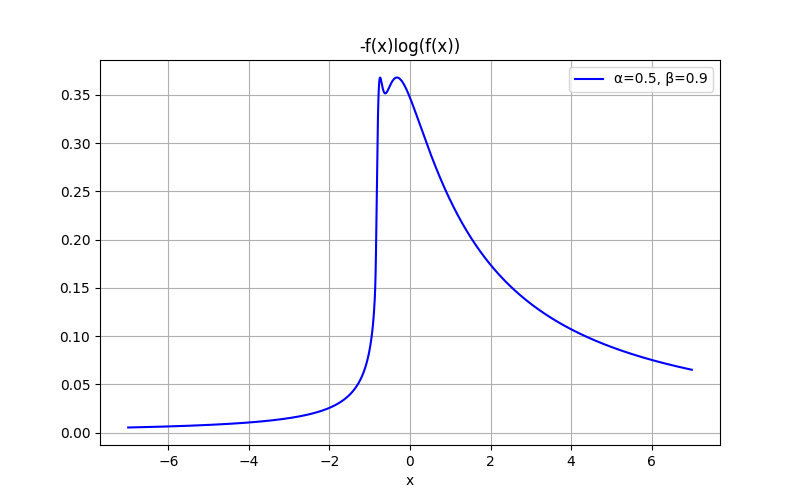
\includegraphics[width=0.9\textwidth]{Erratic.png}
    \caption{Integrand \(-f(x)\log{f(x)}\) for \((\alpha=0.5, \beta=0.9; k=0)\)}
    \label{fig:figure1}
\end{figure}

\subsubsection{Tail Entropy}
%--------------------------------------------
% 2) Right‐tail entropy
%--------------------------------------------
%We need to resolve the remaining half of the problem, now where the integration domain lies in $(-\infty, c_{\tex{left}})\cup(c_{\text{right}},+\infty)$. 
To compute the \textcolor{blue}{(truncated)} tail entropy of \(\alpha\)-stableRV \(X\sim\mathbf{S}(\alpha,\beta;0)\), we will rely on the tail approximation of the pdf \(g{(x)=f_\mathrm{Pareto}(x)}\) (see Property~\ref{pr:tail-approximation}), with its corresponding RV to be \(\mathcal{X}\). The tail entropy as can be approximated as such:
%Note that
%\[
%f(x|\alpha,\beta;0)\sim f_\mathrm{Pareto}(x|\alpha,\beta) \text{ as }x\to\pm\infty
%\]
%or
%\[
%\lim_{x\to\pm\infty}\frac{f(x|\alpha,\beta;0)}{f_\mathrm{Pareto}(x|\alpha,\beta)}=1
%\]
%\begin{flushright}
%\cite{NolanJohnP2020USDM}
%\end{flushright}
%\[
 %     h_{\mathrm{tail}}
  %    = -\int_{-\infty}^{T_{L}}
   %      f(x)\,\log f(x)\,dx
    %  \;-\;\int_{T_R}^{+\infty}
     %    f(x)\,\log f(x)\,dx.
%\]
\[
      h_{\mathrm{tail}}(X)
      \approx h_\mathrm{tail}(\mathcal{X})
\]
%\noindent This is beneficial as a closed-form mathematical expression for \( f_\mathrm{Pareto}(x) \) is available.
%\\\\\\
%\noindent 

We evaluate the right tail entropy \(h_\mathrm{rt}\):
\begin{eqnarray}
h_{\mathrm{rt}}
&\approx& -\int_{T_R}^{\infty}
g(x)\log g(x)\,dx\\
&=& -\int_{T_R}^{\infty}
\alpha\,C_\alpha\,(1+\beta)\,x^{-(1+\alpha)}
\log\bigl(\alpha\,C_\alpha\,(1+\beta)\,x^{-(1+\alpha)}\bigr)\,dx \\
&=& \alpha\,C_\alpha\,(1+\beta)I\,,
\end{eqnarray}
where 
\[
I
= \frac{T_R^{-\alpha}}{\alpha} \left[-\log\bigl[\alpha C_\alpha(1+\beta)\bigr]\,
\;+\;(1+\alpha)\,
\Bigl(\log T_R + \tfrac{1}{\alpha}\Bigr),
\right]\]

\textcolor{blue}{Indeed, we can verify that the actual tail entropy \(h_{rt} \sim \alpha\,C_\alpha\,(1+\beta)\,I \) as \(T_R\to\infty\)}.
%\noindent Since on \([T_R,+\infty)\), \(\;f_{\mathrm{Pareto}}(x)=\alpha\,C_\alpha\,(1+\beta)\,x^{-(1+\alpha)}\):

%\[
%h_\mathrm{right\,tail}
%\approx -\int_{T_R}^{\infty}
%\alpha\,C_\alpha\,(1+\beta)\,x^{-(1+\alpha)}
%\log\!\bigl(\alpha\,C_\alpha\,(1+\beta)\,x^{-(1+\alpha)}\bigr)\,dx.
%\]
%\noindent Since $\alpha\,C_\alpha\,(1+\beta)$ is a constant, pull it out of the integral, and let
%\[
%I_1= -\int_{T_R}^{\infty}x^{-(1+\alpha)}
%\log\!\bigl(\alpha\,C_\alpha\,(1+\beta)\,x^{-(1+\alpha)}\bigr)\,dx
%\]
%\noindent Expanding the log and pulling out the constants gives
%\[
%I_1
%=-\log\bigl[\alpha C_\alpha(1+\beta)\bigr]
%\int_{T_R}^{\infty}
%x^{-(1+\alpha)}\,dx
%\;+\;(1+\alpha)
%\int_{T_R}^{\infty}
%x^{-(1+\alpha)}\,\log x\,dx.
%\]
%Define
%\[
%I_2 \;=\;\int_{T_R}^{\infty}
%x^{-(1+\alpha)}\,\log x\,dx.
%\]
%Integrate \(I_2\) by parts with
%\(\;u=\log x\), \(dv=x^{-(1+\alpha)}\,dx\)\,, so
%\(du=\tfrac{dx}{x}\), 
%\(\;v=\int x^{-(1+\alpha)}dx = -\tfrac{x^{-\alpha}}{\alpha}\).  Thus
%\[
%I_2 = \Bigl[\,-\tfrac{x^{-\alpha}}{\alpha}\,\log x \Bigr] \Bigl|_{T_R}^{\infty}
%\;-\;\int_{T_R}^{\infty}
%\Bigl(-\tfrac{x^{-\alpha}}{\alpha}\Bigr)\,\frac{dx}{x}
%\;=\;
%\frac{T_R^{-\alpha}}{\alpha}
%\Bigl(\log T_R + \tfrac{1}{\alpha}\Bigr).
%\]
%\noindent Hence

%\[
%I_1
%=-\log\bigl[\alpha C_\alpha(1+\beta)\bigr]\,
%\frac{T_R^{-\alpha}}{\alpha}
%\;+\;(1+\alpha)\,
%\frac{T_R^{-\alpha}}{\alpha}
%\Bigl(\log T_R + \tfrac{1}{\alpha}\Bigr),
%\]
%\noindent and therefore
%\[
%h_{\mathrm{right\,tail}}
%=\alpha\,C_\alpha\,(1+\beta)\,I_1
%\]
%\[
%\boxed{
%h_{\mathrm{right\,tail}} = C_\alpha\,T_R^{-\alpha}(1+\beta)\,
%\Bigl[\,(1+\alpha)\bigl(\log T_R+\tfrac{1}{\alpha}\bigr)
%-\log\bigl(\alpha C_\alpha(1+\beta)\bigr)\Bigr].
%}
%\]
%--------------------------------------------
% 3) Left‐tail by symmetry
%--------------------------------------------
Similarly, for the left tail one has to replace 
\(T_R\to\lvert T_{L}\rvert\)
and \(\beta\to-\beta\) due to the reflection property~\ref{reflection-property}. Hence,
\[
h_{\mathrm{lt}}
\approx
C_\alpha\,\lvert T_{L}\rvert^{-\alpha}\,(1-\beta)\,
\Bigl[\,(1+\alpha)\bigl(\log\lvert T_{L}\rvert+\tfrac{1}{\alpha}\bigr)
-\log\bigl(\alpha\,C_\alpha\,(1-\beta)\bigr)\Bigr].
\]
%\noindent We now have a closed-form expression for an approximation of the tail entropy \( h_{\mathrm{tail}} \).
With this, we can proceed to compute the differential entropy of stable distributions, assuming appropriate choices for \( T_{L} \) and \( T_R \). In section~\ref{sec:error}, we answer how these values should be selected, and what are the implications of their choices?

\subsection{Error Analysis}
\label{sec:error}
Estimating the error associated with computing the differential entropy using the method outlined previously is of significant interest. Naturally, since we rely on a numerically generated probability density function (pdf) \( f(x) \), some degree of error will inevitably persist, regardless of the approach employed. For the purpose of this analysis, we will assume that the numerically generated pdf \( f(x) \) is exact, and will focus the investigation on the errors arising from other factors, with particular emphasis on the tail error.

\begin{definition}
We define the relative error $\varepsilon$:
\[
\varepsilon
\;=\;
\frac{\bigl|\,h({X})_{approx.} \;-\; h(X)\bigr|}{h(X)}.
\]
Define the \emph{body error} \(\varepsilon_{\mathrm{body}}\) and the (right/left) \emph{tail error} \(\varepsilon_{\mathrm{tail}}\) similarly, with $h_\mathrm{body}$ and $h_\mathrm{tail}$ instead of \(h\).
\end{definition}

Since closed-form expressions for the differential entropies of Cauchy and L\'evy distributions are available, it is possible to compute the error that results from numerically computed method delineated in the previous section. We vary the cutoff \(T=-T_L=T_R\) (divide the interval symmetrically on the left and right sides), and note the variation of the error \(\varepsilon\), as depicted in figure~\ref{fig:error_vs_cutoff}. As the cutoff \(T\) increases, the overall error \(\varepsilon\) tends to decrease as well.


\subsubsection{Body Error}
Given that the body error $\varepsilon_\mathrm{body}$ arises from integration over a finite interval, it is, in principle, possible to achieve high numerical accuracy using methods such as Gauss-Kronrod adaptive quadrature. This technique refines the integration recursively to satisfy a prescribed error tolerance, limited only by computational precision. Under the assumption that the numerically generated pdf is exact, a body error \( \varepsilon_\mathrm{body} \) on the order of \( 10^{-15} \) is achievable, as demonstrated in the Cauchy distribution case (see figure~\ref{fig:cauchy_error}).


\subsubsection{Tail Error}
The tail error \( \varepsilon_\mathrm{tail} \) arises from approximating the probability density function \( f(x) \) using its asymptotic tail representation. This error is dependent on the cutoff value \( c=T_R \), and it is of interest to establish a relationship between \( \varepsilon_\mathrm{tail} \) and \( c \).
Using the tail approximation for $x > 0$
\begin{equation*}
f(x) \sim g(x)=f_{\mathrm{Pareto}}(x)
= \alpha\,C_\alpha(1+\beta)\,x^{-(1+\alpha)},
\end{equation*}

\iffalse
we obtain for any $k > 0$, 
\begin{equation*}
\frac{f_{\mathrm{Pareto}}(k x)}{f_{\mathrm{Pareto}}(x)}
= \frac{\alpha\,C_\alpha(1+\beta)\,(k x)^{-(1+\alpha)}}
        {\alpha\,C_\alpha(1+\beta)\,x^{-(1+\alpha)}}
= k^{-(1+\alpha)}.
\end{equation*}
Since \(\frac{f(x)}{f_{\mathrm{Pareto}}(x)} \to 1\) as \(x \to \infty\), then \(\frac{f(kx)}{f(x)} \longrightarrow
k^{-(1+\alpha)}\).
%\begin{align*}
%&\text{Since } \frac{f(x)}{f_{\mathrm{Pareto}}(x)} \to 1 
%\quad \text{as } x \to \infty, 
%%\quad \text{and likewise } 
%\frac{f(kx)}{f_{\mathrm{Pareto}}(kx)} \to 1, \\
%&\quad\Longrightarrow\quad
%\frac{f(kx)}{f(x)}
%= \frac{\displaystyle\frac{f(kx)}{f_{\mathrm{Pareto}}(kx)}}
    %    {\displaystyle\frac{f(x)}{f_{\mathrm{Pareto}}(x)}}
%\cdot
%\frac{f_{\mathrm{Pareto}}(kx)}{f_{\mathrm{Pareto}}(x)}
%\;\longrightarrow\;
%k^{-(1+\alpha)}.
%\end{align*}
Indeed, this property can be used to assess how good the tail approximation is at finite \(x\).
%numerically computing
%\[
%\frac{f(2x)}{f(x)}
%\]
%verified that as \(x\to\infty\) (right tail),
%\[
%\frac{f(2x)}{f(x)} \;\longrightarrow\; 2^{-(1+\alpha)}.
%\]
%This gives a sense of how good the tail approximation is at finite \(x\).

\noindent\textbf{Example.}
For \(X\sim S(\alpha=1,\beta=0;\,k=0)\),
\[
\frac{f(2x)}{f(x)} \rightarrow  2^{-(1+\alpha)} = 2^{-2} \quad \text{as }x\to+\infty.
\]

%\noindent\textbf{Numerical values:}
\begin{table}[h!]
\centering
\caption{Tail Approximation Ratio $\frac{f(2x)}{f(x)}$ for increasing values of $x$}
\begin{tabular}{r|l}
\toprule
$x$    & $\displaystyle \frac{f(2x)}{f(x)}$ \\ 
\midrule
4      & 0.26153846153846155 \\
8      & 0.2529182879377432  \\
16     & 0.250731073170317   \\
32     & 0.25018360607767763 \\
64     & 0.2500457235733903  \\
128    & 0.2500114391717566  \\
256    & 0.25000286101203534 \\
512    & 0.2500007152550552  \\
1024   & 0.25000017881389175 \\
2048   & 0.25000004470848086 \\
4096   & 0.2500000111758708  \\
\bottomrule
\end{tabular}
\end{table}
However, it is tricky to bound the tail error knowing the value of $\frac{f(2x)}{f(x)}$. Instead, we introduce the following quantity as defined in \cite{NolanJohnP2020USDM}.
\fi
We denote \(X\) to be a stable RV, and \(\mathcal{X}\) to denote the corresponding Pareto RV. To assess how well \(g(x)\) approximates the tail of \(f(x)\), the following notion present in \cite{NolanJohnP2020USDM} will be useful:
\begin{definition}
Let
\[
L_{\mathrm{pdf}}(x)
\;=\;
L_{\mathrm{pdf}}(x\mid \alpha,\beta)
\;=\;
\frac{f\bigl(x\,|\,\alpha,\beta;0\bigr)}{g\bigl(x\,|\,\alpha,\beta\bigr)}.
\]
For any \(\varepsilon>0\), define the tail‐thresholds
\[
x_{L_{\mathrm{pdf}},\varepsilon}
=\inf\bigl\{\,x>0:|L_{\mathrm{pdf}}(y)-1|\le\varepsilon\;\forall y\ge x\bigr\}
\quad(\text{right side}),
\]
\[
x_{L_{\mathrm{pdf}},\varepsilon}
=\sup\bigl\{\,x<0:|L_{\mathrm{pdf}}(y)-1|\le\varepsilon\;\forall y\le x\bigr\}
\quad(\text{left side}).
\]
\end{definition}

%\begin{definition}
%For any \(\varepsilon>0\), define the tail‐thresholds
%\[
%x_{L_{\mathrm{pdf}},\varepsilon}
%=\inf\bigl\{\,x>0:|L_{\mathrm{pdf}}(y)-1|\le\varepsilon\;\forall y\ge x\bigr\}
%\quad(\text{right side}),
%\]
%\[
%x_{L_{\mathrm{pdf}},\varepsilon}
%=\sup\bigl\{\,x<0:|L_{\mathrm{pdf}}(y)-1|\le\varepsilon\;\forall y\le x\bigr\}
%\quad(\text{left side}).
%\]
%\end{definition}
%\begin{property}
 %We note that \(L_{\mathrm{pdf}}(x)>0\) 
 % \item \(L_{\mathrm{pdf}}(x)>0\) for all \(x\), and \(L_{\mathrm{pdf}}(x)\to1\) as \(x\to\pm\infty\).
  %\item \(L_{\mathrm{pdf}}(x)\) measures the “closeness” between the true pdf and its Pareto tail approximation.
  %\item To distinguish the two errors, we will write \(\varepsilon\) for the tail‐error tolerance, and write \(\varepsilon_1\) when referring to the threshold \(x_{L_{\mathrm{pdf}},\varepsilon_1}\) or the ``closeness" between the true pdf and its Pareto tail approximation.
%\end{itemize}
%\end{property}

We next attempt to bound the relative error on entropy approximation. Let $\varepsilon_1 > 0$ small enough, and let \(x\ge x_{L_{\rm pdf},\varepsilon_1}\) such that 
\[
\log(1\pm\varepsilon_1) \approx \pm\varepsilon_1,
\qquad
(1\mp\varepsilon_1)\,\log(1\pm\varepsilon_1) \approx \pm\varepsilon_1,
\]
and \((1+\varepsilon_1)\,g(x)\le 1\). Using the definition of \(x_{L_{\rm pdf},\varepsilon_1}\), we obtain for \(x\ge x_{L_{\rm pdf},\varepsilon_1}\)
%relate $\varepsilon_1$ and $\varepsilon_{\rm right\,tail}$:
\begin{align*}
%&\forall\,x\ge x_{L_{\rm pdf},\varepsilon_1}: 
%\quad |L_{\rm pdf}(x)-1|\le\varepsilon_1
%\;\Longrightarrow\;
%1-\varepsilon_1 \;\le\; L_{\rm pdf}(x)\;\le\;1+\varepsilon_1,\\
%&\phantom{\Longrightarrow}\quad
%L_{\rm pdf}(x)=\frac{f(x)}{f_{\rm pareto}(x)}
%\;\;\Longrightarrow\;\;
(1-\varepsilon_1)\,g(x) \,\le \, f(x) \,\le\,(1+\varepsilon_1)\,g(x) 
\end{align*}
\[
-\log{[(1 + \varepsilon_1)\,g(x)]} \le -\log f(x) \le - \log{[(1 - \varepsilon_1)\,g(x)]},
\]
%\quad x\ge x_{L_{\rm pdf},\varepsilon_1}.
%\noindent\textit{Remark:} It is reasonable to assume that
%\((1+\varepsilon_1)\,f_{\rm pareto}(x)\le1\) for \(x\ge x_{L_{\rm pdf},\varepsilon_1}\).  
%\\Also use the Taylor approximations:
%\[
%\log(1\pm\varepsilon_1) \approx \pm\varepsilon_1,
%\qquad
%(1\mp\varepsilon_1)\,\log(1\pm\varepsilon_1) \approx %\pm\varepsilon_1.
%\]
%\begin{equation}
%0 
%< (1 - \varepsilon_1)\,f_{\mathrm{Pareto}}(x) 
%\;\le\; f(x) 
%\;\le\; (1 + \varepsilon_1)\,f_{\mathrm{Pareto}}(x) 
%< 1, 
%\quad x \ge x_{L_{\mathrm{pdf}}, \varepsilon_1}
%\end{equation}
%\begin{align*}
%-\infty <\; \log{[(1 - \varepsilon_1)\,f_{\mathrm{Pareto}}(x)]} \;\le\; \log{f(x)} \;\le\; \log{[(1 + \varepsilon_1)\,f_{\mathrm{Pareto}}(x)]} < 0
%\end{align*}
%\begin{equation}
%0<\,-\log{[(1 + \varepsilon_1)\,f_{\mathrm{Pareto}}(x)]} \le -\log{f(x)} \le - \log{[(1 - \varepsilon_1)\,f_{\mathrm{Pareto}}(x)]} < +\infty
%\end{equation}
%\\
which implies
\[
-(1 - \varepsilon_1)\,g(x)\,
\log\bigl[(1 + \varepsilon_1)\,g(x)\bigr]
\leq - f(x) \log f(x)
\leq - (1 + \varepsilon_1)\,g(x)\,
\log\bigl[(1 - \varepsilon_1)\,g(x)\bigr]
\]

Using Taylor approximation,
\begin{equation*}
- \varepsilon_1(1-\varepsilon_1)\,g(x)-(1-\varepsilon_1)\,g(x)
\log g(x)
\lesssim -f(x)\,\log f(x) \lesssim 
 +\varepsilon_1(1 + \varepsilon_1)\,g(x)-(1+\varepsilon_1)\,g(x)
\log g(x)
\end{equation*}

Integrating both sides over 
\( x \in [x_{L_{\mathrm{pdf}},\varepsilon_1},\,+\infty) \), we obtain:
\begin{equation*}
(1 - \varepsilon_1) \left(-\varepsilon_1 \overline{G}(x_{L_{\mathrm{pdf}},\varepsilon_1})+h_{\rm Pareto,rt}\right)\lesssim h_{\rm rt}\lesssim (1 + \varepsilon_1) \left(\varepsilon_1 \overline{G}(x_{L_{\mathrm{pdf}},\varepsilon_1})+h_{\rm Pareto,rt}\right),
\end{equation*}
where \(\overline{G}\) corresponds to the survival function of \(g(x)\). Therefore,
\begin{equation*}
\left|\frac{h_{\rm rt}(\mathcal{X}) \, -\, h_{\rm rt}(X)}{h_{\rm rt}{(\mathcal{X})}} \right| 
\;\lesssim\; 
\varepsilon_1 \left| \frac{\overline{G}(x_{L_{\mathrm{pdf}},\varepsilon_1})}{h_{\rm Pareto,rt}}+1 \right| \triangleq \varepsilon'_{\rm right}. 
\end{equation*}

\textcolor{blue}{
Note that for \(x_L > \max\{x_m, \alpha\}\),
\begin{align*}
\varepsilon_1 \left| \frac{\overline{G}(x_{L_{\mathrm{pdf}},\varepsilon_1})}{h_{\rm rt}(\mathcal{X})} + 1 \right|  &= \varepsilon_1 \left( \frac{1}{\alpha \log\frac{x_L}{x_m} + \log{\frac{x_L}{\alpha} + \frac{\alpha + 1}{\alpha}}}+1 \right)
< \varepsilon_1 \left( \frac{\alpha}{\alpha +1 } + 1 \right) \le\frac{5}{3}\varepsilon_1
\end{align*}
where \( x_L := x_{L_\mathrm{pdf}} \) and \( x_m := [C_\alpha (1+\beta)]^{\frac{1}{\alpha}}\).
\\
}

\textcolor{blue}{The above succesfully establishes a practical bound on the tail error that may result from the approximation which depends on how well the tail of the Pareto distribution approximate the the tail of the actual probability distribution} (refer to figure~\ref{fig:figure4}).

We have successfully established a bound on the tail error, which provides a means of selecting an appropriate cutoff value to ensure that the tail entropy is computed to within a desired level of accuracy.
\begin{figure}[h!]
    \centering
    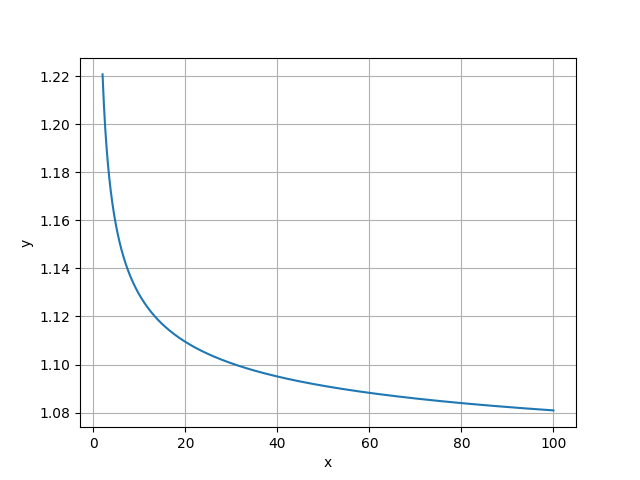
\includegraphics[width=0.75\textwidth]{Figure_3.png}
    \caption{\(\frac{\overline{G}(x)}{h_{\rm Pareto,[x,+\infty)}} + 1\) as a function of $x$ for standard Cauchy.}
    \label{fig:figure4}
\end{figure}
\noindent

\textcolor{blue}{Alternatively, the asymptotic (absolute) tail error may be determined:
\begin{equation*}
    h_{[T,\infty)}(X)-h_{[T,\infty)}(\mathcal{X})\sim CT^{-k}\log(T)
\end{equation*}
where \(C\) and \(k\) are some constants, and \(X\) is the RV corresponding to an alpha-stable distribution and \(\mathcal{X}\) is the RV corresponding to the appropriate Pareto distribution. The details are presented in the following Lemma~\ref{lem:tail-entropy-trunc-err}.
}

\begin{lemma}[Leading entropy-kernel truncation error]\label{lem:tail-entropy-trunc-err}
Let $\{\varphi_n\}_{n\ge1}$ be an asymptotic scale as $x\to a$ with
\[
\varphi_{n+1}(x)=o(\varphi_n(x)), \qquad \varphi_1(x)\to0^+,
\]
and suppose that
\[
f(x)\sim \sum_{n=1}^\infty a_n\varphi_n(x)
\quad \text{as } x\to a,
\]
in the sense of Copson (see~\ref{def:asymptotic-scale}~and~\ref{def:asymptotic-expansion}), with \(a_1>0\) and \(a_2\neq0\).  
Define the leading-term approximation
\[
g(x):=a_1\varphi_1(x).
\]
Then the entropy kernel satisfies
\[
f(x)\log f(x)-g(x)\log g(x)
\sim
a_2\,\varphi_2(x)\,\log\left(a_1\varphi_1(x)\right),
\qquad x\to a.
\]
Equivalently,
\[
f(x)\log f(x)-g(x)\log g(x)
=
a_2\,\varphi_2(x)\,\log\varphi_1(x)
+
O\!\left(\varphi_2(x)\right),
\qquad x\to a.
\]
\end{lemma}
In particular, for \(\alpha\)-stable distribution \(f(x)\) with \(g(x)\) the first term in asymptotic expansion as given in \ref{pr:tail-approximation}~and~\ref{pr:asymptotic-expansion}, one has
\[
-f(x)\log f(x)+g(x)\log g(x)
\sim
(1+\alpha)D_2^+\,x^{-(1+2\alpha)}\log x \quad \text{as }x\to\infty.
\]
assuming \(D_2^+\neq0\).
\begin{proof}
By assumption,
\[
f(x)\sim \sum_{n=1}^\infty a_n\varphi_n(x)
\quad \text{as } x\to a,
\]
in the sense of Copson, with $\varphi_{n+1}(x)=o(\varphi_n(x))$ and
$\varphi_1(x)\to0^+$.  Define
\[
g(x):=a_1\varphi_1(x).
\]

Then $f$ may be written as a perturbation of $g$:
\[
f(x)=g(x)\bigl(1+\varepsilon(x)\bigr),
\qquad
\varepsilon(x)
=
\frac{a_2}{a_1}\frac{\varphi_2(x)}{\varphi_1(x)}
+
O\!\left(\frac{\varphi_3(x)}{\varphi_1(x)}\right),
\qquad x\to a.
\]
In particular, $\varepsilon(x)\to0$.

Using the Taylor expansion of the logarithm at $1$,
\[
\log(1+\varepsilon)
=
\varepsilon-\tfrac12\varepsilon^2+O(\varepsilon^3),
\qquad \varepsilon\to0,
\]
we obtain
\[
\log f(x)
=
\log g(x)
+
\varepsilon(x)
-
\tfrac12\varepsilon(x)^2
+
O(\varepsilon(x)^3).
\]

Multiplying by $f(x)=g(x)(1+\varepsilon(x))$ yields
\[
\begin{aligned}
f(x)\log f(x)
&=
g(x)\log g(x)
+
g(x)\varepsilon(x)\log g(x)
+
g(x)\varepsilon(x)
+
O\bigl(g(x)\varepsilon(x)^2\log g(x)\bigr).
\end{aligned}
\]

Subtracting \(g(x)\log g(x)\)gives
\[
f(x)\log f(x)-g(x)\log g(x)=g(x)\varepsilon(x)\log g(x)
+g(x)\varepsilon(x)+
O\left(g(x)\varepsilon(x)^2\log g(x)\right).
\]

Since $g(x)=a_1\varphi_1(x)$ and
$\varepsilon(x)=\frac{a_2}{a_1}\frac{\varphi_2(x)}{\varphi_1(x)}+o\!\left(\frac{\varphi_2}{\varphi_1}\right)$,
we have
\[
g(x)\varepsilon(x)
=
a_2\varphi_2(x)
+
o\!\left(\varphi_2(x)\right),
\]
and
\[
g(x)\varepsilon(x)\log g(x)
=
a_2\varphi_2(x)\log\bigl(a_1\varphi_1(x)\bigr)
+
o\!\left(\varphi_2(x)\log\varphi_1(x)\right).
\]
Because $\log\varphi_1(x)\to-\infty$ as $x\to a$, the logarithmic term dominates,
and therefore
\[
f(x)\log f(x)-g(x)\log g(x)
\sim
a_2\,\varphi_2(x)\,\log\bigl(a_1\varphi_1(x)\bigr),
\qquad x\to a.
\]

Equivalently,
\[
f(x)\log f(x)-g(x)\log g(x)
=
a_2\,\varphi_2(x)\,\log\varphi_1(x)
+
O\!\left(\varphi_2(x)\right),
\qquad x\to a,
\]
which completes the proof.
\end{proof}

\begin{corollary}\label{cor:tail-error-bound}
Let \(X\sim\mathbf{S}(\alpha,\beta;0)\) \(\alpha\)-stable r.v., and \(\mathcal{X}\) the RV corresponding to the appropriate Pareto distribution \(g(x)\).\\
Assume \(D_2^+\neq0\) (see Property~\ref{pr:asymptotic-expansion}). As \(T\to\infty\):
\begin{equation}
    h_{[T,\infty)}(X)-h_{[T,\infty)}(\mathcal{X})=\frac{1+\alpha}{2\alpha}D_2^+T^{-2\alpha}\log(T)+O(T^{-2\alpha})
\end{equation}
\textit{Note:} If \(D_2^+=0,\) a simple redefinition of asymptotic scale (in which \(\varphi_n\) with its corresponding coefficients \(D_n^+=0\) are dropped from the asymptotic scale) such that the redefined asymptotic scale has \(D_n^+\neq0\) for all \(n\), in particular \(D_2^+\neq0\) can be done. Then apply Lemma~\ref{lem:tail-entropy-trunc-err}. (The case \(\beta=-1\) is ignored here). 
\end{corollary}
A straightforward example of Corollary~\ref{cor:tail-error-bound} for Cauchy distribution \(\mathbf{S}(1,0;0)\) is presented.

\begin{example}
Let \(X\sim\mathbf{S}(1,0;0)\) Cauchy distribution, and \(\mathcal{X}\) as usual with \(f\) and \(g\) as their corresponding pdfs. From Example~\ref{ex:Cauchy-asymp-exp}, the second non-zero coefficient in its asymptotic expansion is \(D_2^+=-\frac{1}{\pi}\) with \(\varphi_2(x)=x^{-4}\). By Lemma~\ref{lem:tail-entropy-trunc-err}, as \(x\to\infty,\)
\begin{equation*}
    -f(x)\log f(x)+g(x)\log g(x)=-2\,D_2^+x^{-4}\log{x}+O(x^{-4})
\end{equation*}
Therefore, as \(T\to\infty\),
\begin{equation}\label{eq:Cauchy-tail-ent-error}
    h_{[T,\infty)}(X)-h_{[T,\infty)}(\mathcal{X})=\frac{2}{3\pi}T^{-3}\log{T}+O(T^{-3}).
\end{equation}
The preceding equation~\ref{eq:Cauchy-tail-ent-error} implies the rate at which the (absolute) tail error decays for Cauchy. If the assumption that \(\varepsilon_{body}\approx 0\) a negligible constant w.r.t. \(\varepsilon_{tail}\) can be made (almost independent of \(T\) as \(T\) increases), then relative error \(\varepsilon=\Theta(T^{-3}\log{T)}\).
For large T, when the relative error \(\varepsilon\) is plotted as a function of \(T\) on a log-log~scale, we expect a linear relation with slope \(\approx-3\). The plot of error as a function of cutoff T from numerical computations (see~\ref{fig:cauchy_error}) does indeed exhibit a slope close to \(-3\).
\end{example}

A similar analysis can be done for L\'evy distribution, \(X\sim\mathbf{S}(0.5,1;0)\). Noting that \(D_2^+=0\) as presented in Property \ref{pr:asymptotic-expansion}, the asymptotic scale needs to be redefined to ignore the vanishing coefficients. Indeed with the same assumptions made in the Cauchy case, we expect to notice a slope \(\approx-1.5\) when plotting relative error \(\varepsilon\) for a large enough cutoff \(T\), which can be verified by plot~\ref{fig:levy_error}.


\begin{figure}[h!]
    \centering
    \begin{subfigure}[b]{0.49\textwidth}
        \centering
        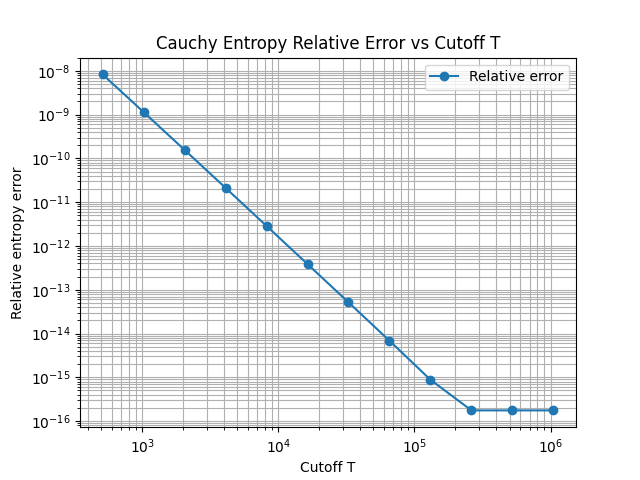
\includegraphics[width=\textwidth]{Cauchy_rel_error_vs_cutoff_T.png}
        \caption{``Cauchy'' $(\alpha=1,\beta=0; k=1)$}
        \label{fig:cauchy_error}
    \end{subfigure}
    \hfill
    \begin{subfigure}[b]{0.49\textwidth}
        \centering
        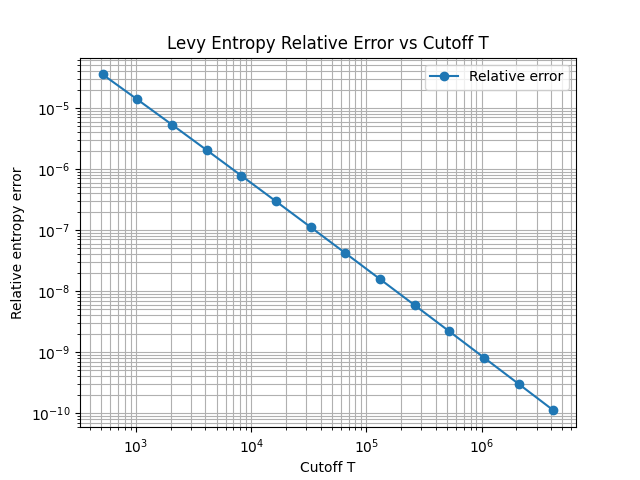
\includegraphics[width=\textwidth]{Levy_rel_error_vs_cutoff_T.png}
        \caption{``L\'evy'' $(\alpha=0.5,\beta=1; k=1)$}
        \label{fig:levy_error}
    \end{subfigure}
    \caption{Relative error $\varepsilon$ as a function of cutoff \(T\) for Cauchy and L\`evy distributions}
    \label{fig:error_vs_cutoff}
\end{figure}

\textit{Note 1:} To generate the above plots, the closed-form expressions for the PDF \( f(x) \) of the Cauchy and L\`evy distributions were used.

\textit{Note 2:} Certain large values of T may fail to compute the body entropy properly, and will yield significant error in that case.

\section{Randomized QMC Method using Sobol Sequences}
Alpha Stable distributions lack closed form expressions for their PDF in most cases; however, there are known methods to sample from an Alpha Stable distribution and to evaluate the PDF numerically such as the algorithm presented in \cite{ChambersJ.M.1976AMfS} to sample and the methods presented in \cite{NolanJohnP.1997Ncos} to evaluate the PDF numerically. For these purposes, we are motivated to compute the differential entropy using Monte Carlo simulation.
\subsection{Overview On Monte Carlo Simulation}
In Monte Carlo simulation, the quantity of interest is interpreted in the context of a stochastic model and then computed by random sampling. Let \(X\sim\mathbf{S}(\alpha,\beta;k)\) with PDF \(f(x)\) and CDF \(F(x)\) then from \eqref{definition of differential entropy} we can see that
\begin{equation}
h(X) =-\int_{-\infty}^{\infty} f(x) \log f(x) \, dx 
= -\int_0^1 \log(f(F^{-1}(u))) \, du
=\int_0^1 g(u)du 
=\mathbb{E}[g(U)] \qquad U \sim \mathcal{U}[0,1],
\end{equation}
where we used the change of variable \(u = F(x)\) and where \(g(u) \triangleq -\log(f(F^{-1}(u)))\) and \(U\sim\mathcal{U}[0,1]\) means that \(U\) is distributed uniformly on the interval \([0,1]\). By the SLLN, for a large number of samples \(u_1,u_2,\ldots, u_n\) sampled from \(U\sim\mathcal{U}[0,1]\), \begin{equation}\label{Monte Carlo Simulation}
h(X)=\mathbb{E}[g(U)]\approx \frac{1}{n}\sum_{i=1}^n g(u_i) 
\end{equation}
This method seems promising for computing the differential entropy; however, the mean square error (MSE) is \(\Theta\left(\frac{1}{n}\right)\)\cite{NiederreiterHarald1992Rnga} which is a probabilistic error bound that is slowly decaying. Since we are interested in deterministic error bounds that are fast decaying, the classical Monte Carlo method is unattractive for the purpose of computing differential entropy.
There are several methods to achieve faster decaying Monte Carlo errors that are discussed in \cite{NiederreiterHarald1992Rnga}. One of these methods is called the Quasi-Monte Carlo (QMC) method, which we discuss in the following.
\subsection{The Quasi-Monte Carlo Method}
In the QMC method, we estimate the integral using the same sum presented in \eqref{Monte Carlo Simulation} except that the points \(u_1,u_2,\ldots,u_n\) are deterministic points that are chosen in such a way to make the error decay much faster. We will see throughout this paper that choosing these points to be \emph{well spread} throughout the interval \([0,1]\) can achieve  a faster decaying error.In usual Monte Carlo simulation, the sum converges to the quantity of interest by the SLLN. With the QMC method convergence is guaranteed by another criterion which we discuss in the following. Using the same notation as in \cite{NiederreiterHarald1992Rnga}, for \(s\geq 1\), let \(\bar{I}^{s}=[0,1]^s\) be the \(s\)-dimensional unit cube. Let  \(J\subset \bar{I}^{s}\) and \(x\in \bar{I}^{s}\) then the characteristic function of \(J\) is given by
\begin{equation}
    c_J(x) =
    \begin{cases}
        1 & x\in J \\
        0 & x\notin J
     \end{cases}
\end{equation}
\begin{definition}\label{counting finite}
Let \(\mathcal{P}\) be a point set consisting of $\mathbf{x}_1,\mathbf{x}_2,\cdot\cdot\cdot\mathbf{x}_n\in\bar{I}^{s} $.  We  interpret a
``point set" in the sense of the combinatorial notion of ``multiset," that is a set in, which the multiplicity of elements matters, so duplicates are not omitted. For an arbitrary \(B\subset\bar{I}^{s}\) the counting function that gives the number of elements of \(\mathcal{P}\) that are in $B$ is given by  
\begin{equation}
 A(B,\mathcal{P})=\sum_{i=1}^n c_B(x_i)
\end{equation}  
\end{definition}

\begin{definition}\label{counting infinite}
Let \(x_1,x_2,\ldots\) be a sequence of real numbers, let \(n\) be a positive integer and let \(E\subset [0,1)\). The counting function \(A(E;n)\) is the number of terms \(x_i,1\leq i\leq n\) such that \(x_i\in E\) 
\end{definition}

\begin{definition}\label{unifromly distributed} Let \(s=1\). A sequence of points \(u_1,u_2,\ldots\) is said to be \emph{uniformly distributed modulo 1} (u.d mod 1) in the interval \([0,1]\) if for all \(a,b\in\mathbb{R}\), \(0\leq a<b\leq1\), we have  
    \begin{equation}
        \lim_{n\to\infty}\frac{A([a,b),n)}{n}=b-a
    \end{equation}
\end{definition}

\begin{theorem}\label{thm: criterion for QMC convergence}
    A sequence \(u_1,u_2,\ldots\) of real numbers is u.d mod 1 if and only if for every real-valued continuous function \(f\) defined on the closed unit interval \(\bar{I}=[0,1]\) we have  
    \begin{equation}
        \lim_{n\to\infty}\frac{1}{n}\sum_{i=1}^n f(u_i)=\int_{\bar{I}}f(u)du
    \end{equation}
\end{theorem}

\noindent Definition \ref{counting finite} is taken from \cite{NiederreiterHarald1992Rnga} and Definitions \ref{counting infinite}, \ref{unifromly distributed}, and Theorem \ref{thm: criterion for QMC convergence} are taken from \cite{alma991015801878809621}; the proof of Theorem \ref{thm: criterion for QMC convergence} can be found in \cite{alma991015801878809621}. Note that definition \ref{unifromly distributed} and Theorem \ref{thm: criterion for QMC convergence} provide a criterion to know if the sum converges to the desired quantity. However, it is difficult to verify the criterion presented in Theorem \ref{thm: criterion for QMC convergence}, so we will introduce an alternative way to verify this condition and thus attain convergence, but first we need to present some preliminaries on discrepancy theory. 
\subsection{Preliminaries on Discrepancy Theory}
In this section,we list some definitions and results from discrepancy theory which are taken from \cite{NiederreiterHarald1992Rnga}.
 \begin{definition}
 Let \(\mathcal{J}^{\ast}\) be the family of all sub-intervals of \({I}^{s}\) of the form \(\prod_{i=1}^{s} [0,u_i)\). The \emph{star discrepancy} \(D_n^{\ast}(\mathcal{P})\) is defined as 
\begin{equation}
     D_n^{\ast}(\mathcal{P})=\sup_{\; B\in \mathcal{J}^{\ast}}\left\lvert \frac{A(B,\mathcal{P})}{n}-\lambda_s(B)\right\rvert
\end{equation}
\end{definition}

\noindent where \(\lambda_s\) denotes the \(s\)-dimensional Lebesgue measure.

\begin{definition} 
Let \(\mathcal{J}\) be the family of all sub-intervals of \({I}^{s}\) the form \(\prod_{i=1}^{s} [u_i,v_i)\). The \emph{extreme discrepancy} \(D_n(\mathcal{P})\) is defined as 
\begin{equation}
    D_n(\mathcal{P})=\sup_{\; B\in \mathcal{J}}\left\lvert \frac{A(B,\mathcal{P})}{n}-\lambda_s(B)\right\rvert
\end{equation}
\end{definition}

\noindent Often, extreme discrepancy is simply referred to as \emph{discrepancy}, and we will use the term \emph{discrepancy} throughout this work. Note that discrepancy is larger than the star discrepancy because it considers much more sub-intervals than the star version. This is highlighted in the following lemma that is proven in \cite{NiederreiterHarald1992Rnga}.

\begin{lemma} 
For any \(\mathcal{P}\) consisting of points in \(\bar{I}^{s}\) we have
\begin{equation}\label{discrepancy and extreme discrepancy}
D_n^{\ast}(\mathcal{P})\leq D_n(\mathcal{P}) \leq 2^{s} D_n^{\ast}(\mathcal{P})
\end{equation}
\end{lemma}

\noindent We can see that discrepancy is a `measure' of how close is the point set under consideration to the uniform distribution mod 1 where smaller values of discrepancy are associated with a point set that is closer to a uniform distribution mod 1. In fact, we can check if a sequence is uniformly distributed by examining its discrepancy. We make this precise in the following theorem whose proof is in \cite{alma991015801878809621}.

\begin{theorem}\label{discrepancy equivalent}
    A sequence $\{x\}_{n=1}^{\infty}$ is u.d mod 1 if and only if $\lim_{n\to\infty}D_n(\{x_n\})=0$ where $D_n(\{x_n\})$ is the discrepancy of the first $n$ points of the sequence. 
\end{theorem}

\noindent From Theorems \ref{thm: criterion for QMC convergence} and \ref{discrepancy equivalent}, we require sequences that satisfy $\lim_{n\to\infty}D_n(\{x_n\})=0$, and we will also  see that the discrepancy of the point set that we are using to sample from our alpha-stable distribution affects the upper bound of the error in the entropy estimate.Therefore, we would like to use point sets that have low discrepancy and whose discrepancy is 0 in the limit.For this purpose, we use a special type of point sets called $(t,m,s)$ nets that satisfy these properties.The following defintions are taken from \cite{NiederreiterHarald1992Rnga}.

\begin{definition}
 Let \(s\geq 1\) and \(b\geq 2\). A subinterval \(E\) of \(I^s\) of the form \(E=\prod_{i=1}^s[a_ib^{-d_i},(a_i+1)b^{-d_i})\) where \(a_i,d_i\in\mathbb{Z},\; d_i\geq 0,\;0\leq a_i<b^{d_i}\) for \(1\leq i\leq s\) is called an elementary interval in base \(b\).
 \end{definition}
 
\begin{definition}
Let $0\leq t\leq m$ be integers. A $(t,m,s)$-net in base $b$ is a point set $\mathcal{P}$ of $b^m$ points in $I^s$ such that $A(E;\mathcal{P})=b^t$ for every elementary interval $E$ in base b with $\lambda_s(E)=b^{t-m}$.
\end{definition}

\begin{definition}
Let $t\geq 0$ be an integer. A sequence $\mathbf{x}_0,\mathbf{x}_1,\ldots$ of points in $I^s$ is a $(t,s)$-sequence in base $b$ if , for all integers $k\geq 0$ and $m> t$, the point set consisting of the $\mathbf{x}_n$ with $kb^m\leq n< (k+1)b^m$ is a $(t,m,s)$ net in base $b$.
\end{definition}

\noindent There are many well known $(t,s)$ sequences; Sobol' introduced $(t,s)$ sequences in base 2 in 1967,  Faure introduced constructions of $(0,s)-$sequences in a prime base $b$ with $b\geq s$ in 1982, and Niederreiter provided a unifying approach to construct these sequences using polynomial arithmetic over finite fields. We also note that the value of $t$ for Sobol Sequences does not depend on the number of sampled points\cite{DickJosef2010D}.For our computational task, we chose Sobol Sequences because they can be implemented in a simple and efficient way. In particular, we use the Sobol Sequence implementation provided in the \texttt{Scipy} QMC numerical package. In Appendix~\ref{app:sobol}, we present an algorithm to generate Sobol Sequences.In the following, we discuss a discrepancy bound for Sobol Sequences, which was proven in \cite{DickJosef2010D}.

\begin{theorem}
\label{th:discb2}
The star discrepancy of  a $(t,m,s)$-net $\mathcal{P}$ in base 2 satisfies \begin{equation}
    2^m D^{\ast}_{2^m}(\mathcal{P})\leq 2^t \sum_{i=0}^{s-1} \binom{m-t}{i}
\end{equation} 
\end{theorem}

\noindent Applying theorem 1 for $s=1$, and using the fact that for a $(t,m,1)$ net we have $n=2^m$,  we get that for a $(t,m,1)$ net in base 2
\begin{equation}\label{discrepancy bound}
    D_n^{\ast}(\mathcal{P})\leq \frac{2^t}{n}
\end{equation}
From equations \eqref{discrepancy bound} and inequality \eqref{discrepancy and extreme discrepancy}, we can see that for Sobol Sequences $\lim_{n\to\infty}D_n(\{x_n\})=0$ hence  by Theorem \ref{discrepancy equivalent} Sobol Sequences are u.d mod 1 and by Theorem \ref{thm: criterion for QMC convergence} the quasi-Monte Carlo sum converges to the desired quantity, so Sobol Sequences are a good candidate for QMC integration.We had previously discussed how the discrepancy of the point set affects the bound on the error of the entropy estimate. We make this precise in the following section where the resulting error given by the Koksma-Hlawka inequality (Theorem~\ref{th:KH}) is of particular importance.

\begin{definition}
    Let $g$ be a function that has continuous partial derivatives of order $1,2,\ldots, s$ on $\bar{I}^{s}$ . The variation of $g$ in the sense of Vitali is given by \begin{equation}
    V^{(s)}(g)=\int_0^1 \cdot\cdot\cdot\int_0^1 \left\lvert \frac{\partial^{s}g}{\partial u_1 \partial u_2\cdot\cdot\cdot\partial u_s}\right\rvert du_1du_2\cdot\cdot\cdot du_s
    \end{equation}
\end{definition}

\begin{definition}
 For $1\leq k\leq s$ and $1\leq i_1 <i_2<\cdot\cdot\cdot< i_k\leq s$, Let $V^{(k)}(g;i_1,\cdot\cdot\cdot,i_k)$ be the variation in the sense of Vitali of the restriction of $g$ to the $k$-dimensional face $\{(u_1,\cdot\cdot\cdot,u_s)\in \bar{I}^{s}: u_j=1 \text{ for } j\neq i_1,\cdot\cdot\cdot, i_k\}$. Then the variation of $g$ on $\bar{I}^s$ in the sense of Hardy and Krause is given by \begin{equation}\label{Variation in the sense of Hardy and Krause}
     V(g)=\sum_{k=1}^s \sum_{1\leq i_1 <i_2<\cdot\cdot\cdot< i_k\leq s}V^{(k)}(g;i_1,\cdot\cdot\cdot,i_k)
 \end{equation}  We say that $g$ is of
 bounded variation in the sense of Hardy and Krause (BVHK) if $V(g)$ is finite.The Koksma-Hlawka, inequality relates the error of the QMC estimate to the variation in the sense of Hardy and Krause.The proof of the inequality can be found in  \cite{alma991015801878809621} and we state it in the following theorem. 
 \end{definition}

\begin{theorem}
\label{th:KH}
Let ${I}^{s}=[0,1)^s$ . If $g$ has a bounded variation $V(g)$ on ${I}^{s}$ in the sense of Hardy and Krause, then for any $\mathbf{x}_1,\mathbf{x}_2,\cdot\cdot\cdot,\mathbf{x}_n\in I^s$, we have
    \begin{equation}\label{Koksma Hlawka Inequality}
    \left\lvert \frac{1}{n}\sum_{i=1}^ng(\mathbf{x}_i) -\int_{\bar{I}^s} g(\mathbf{x})d\mathbf{x}  \right\rvert\leq V(g)D^{\ast}(\mathbf{x}_1,\mathbf{x}_2,\ldots,\mathbf{x}_n)
    \end{equation}
where $D^{\ast}(\mathbf{x}_1,\mathbf{x}_2,\ldots,\mathbf{x}_n)$ is the star discrepancy of the used points.
\end{theorem}
 
 \noindent There are several problems that arise when we want to apply this inequality to obtain the error of our QMC estimate using Sobol Sequences.In the following section, we discuss the problems, their corresponding solutions, and the technicalities of implementing such solutions.
\subsection{Challenges of Applying the Koksma-Hlawka Inequality} 
\subsubsection{Unbounded Variation in the sense of Hardy and Krause}
The first problem that we encounter while applying inequality \eqref{Koksma Hlawka Inequality} is that in general, the PDF of alpha stable distributions do not have a finite variation in the sense of Hardy and Krause.For instance, consider the normalized Cauchy  distribution whose PDF $f(x)$ is given by  \begin{equation}
    f(x)=\frac{1}{\pi}\frac{1}{1+x^2}
\end{equation}
The variation in the sense of Hardy and Krause for $s=1$ is given by \eqref{Variation in the sense of Hardy and Krause} as follows \begin{equation}
    V(g)=\int_{0}^1\left\lvert g^{\prime}(u)\right\rvert du \qquad g(u)=-\log\left(f(F^{-1}(u))\right)  
\end{equation}
Changing the integral back to the entire support of the distribution, we have $x=F^{-1}(u)\Rightarrow F(x)=u $\\ $\Rightarrow f(x)dx=du$. Then we have \begin{align*}
    V(g)&=\int_{0}^1\left\lvert g^{\prime}(u)\right\rvert du =\int_0^1\left\lvert \frac{f^{\prime}(F^{-1}(u))}{f(F^{-1}(u))}\frac{d}{du}\left[F^{-1}(u)\right]\right\rvert du=\int_0^1\left\lvert \frac{f^{\prime}(F^{-1}(u))}{f(F^{-1}(u))}\frac{1}{F^{\prime}(F^{-1}(u))}\right\rvert du\\
    &=\int_0^1\left\lvert \frac{f^{\prime}(F^{-1}(u))}{f^2(F^{-1}(u))}\right\rvert du=\int_{-\infty}^{\infty}\left\lvert \frac{f^{\prime}(x)}{f^2(x)}\right\rvert f(x)dx=\int_{-\infty}^{\infty}\left\lvert \frac{f^{\prime}(x)}{f(x)}\right\rvert dx=\int_{-\infty}^{\infty}\frac{2\lvert x\rvert }{1+x^2} dx  
\end{align*}
and the integral in the last equality diverges. Therefore, we cannot apply the Koksma-Hlwaka Inequality to Alpha Stable distributions directly. We will solve this problem by truncating $g(u)$ to $\hat{g}(u)$ so that the integral above is finite.We will present the truncation region and justify our choice of this region throughout this paper. 
\subsubsection{The Problem with Zero}
From Appendix \ref{app:sobol}, we know that the first point in the Sobol Sequence is zero, but this means that \begin{equation}
    \lim_{u\to0^{+}} g(u)=-\lim_{u\to0^{+}}\log\left(f(F^{-1}(u))\right)=-\lim_{x\to -\infty}\log(f(x))=-\lim_{t\to 0^{+}}\log(t)=+\infty
\end{equation} 
hence the sum of the entropy estimate  diverges. Simply removing the first Sobol point does not solve the problem becuase the resulting point set that we are using for numerical integration is no longer a \((t,m,s)\) net; on the consequences of removing the first point, we refer the reader to \cite{OwenArtB2021Odtf}. In the following, we present two solutions to solve this problem, a deterministic solution, and a randomized one.
\subsubsection{First Solution: Shifting}
The first solution is to shift all the generated points by adding $\frac{1}{2n}$ to all the sampled points, so none of the points will be zero. The discrepancy bound in \eqref{discrepancy bound} becomes slightly looser as discussed in the following.
 \begin{theorem}
  \label{th:r5}
 Let $\mathcal{P}=\{x_1,x_2\ldots,x_{n}\}$ be a $(t,m,1)$-net of Sobol points. Let $\mathcal{P}_{\text{shifted}}$ be the resulting set of points after adding $\frac{1}{2n}$ to each point in $\mathcal{P}$ Then the star discrepancy  $D^{\ast} _n(\mathcal{P}_{\text{shifted}})$ satisfies: 
 \begin{equation}
 \label{same bound two}
     D^{\ast} _n(\mathcal{P}_{\text{shifted}}) \leq \frac{1+2^{t}}{n}
 \end{equation}
\end{theorem}

\begin{proof}
Let $\epsilon=\frac{1}{n}$ and let $\delta_{i}=\frac{1}{2n}$ then $\delta_{i}< \epsilon, \;\forall \, 0\leq i\leq n-1$. In addition $\forall\; 0\leq i\leq n-1$  
 we have \begin{align*}
    x_{i}+\delta_{i}&=x_{i}+\frac{1}{2n}\\
    &\leq 1-\frac{1}{n}+\frac{1}{2n}&& \text{ (Lemma~\ref{lem:r1})}\\
    &= 1-\frac{1}{2n}<1
\end{align*}
\noindent Therefore,Theorem~\ref{th:shift} in Appendix~\ref{app: Owen Scrambling} applies and we have that $\lvert D_n^{\ast}(\mathcal{P}) - D_n^{\ast}(\mathcal{P}_{\text{shifted}})\rvert \leq \frac{1}{n}$  then \begin{align*}
D_n^{\ast}(\mathcal{P}_{\text{shifted}})&\leq \frac{1}{n} + D_n^{\ast}(\mathcal{P})\\
&\leq\frac{1}{n}+\frac{2^t}{n}&& (\ref{discrepancy bound})\\
&=\frac{1+2^{t}}{n}\end{align*}
\end{proof}
\subsubsection{Second Solution: Owen Scrambling-Randomized QMC}
The second solution is to use an algorithm that randomizes the points that we are using called \textit{Owen Scrambling} which is presented in \cite{OwenArtB.1995RP(m} .This algorithm is very helpful because randomization can remove the point zero with high probability. We will make this statement more precise later on in this work. In Appendix \ref{app: Owen Scrambling}, we discuss the scrambling algorithm presented \cite{OwenArtB.1995RP(m}.The theoretical scrambling algorithm, requires considering an infinite number of additional bits, but for implementation purposes we, we have to use a finite number of additional bits which we denote by $k$ throughout this paper, and we will use the term approximately Owen Scrambled with $k$ additional bits for the point set obtained by scrambling using $k$ additional bits.This computational method  falls under the category of Randomized-QMC(RQMC). Another natural problem that presents itself is whether the discrepancy bound in \eqref{discrepancy bound} is preserved after scrambling.In the following, we present the merits of \textit{Owen Scrambling} wich are that the resulting points are distributed as $\mathcal{U}[0,1)$ and that the complexity of the discrepancy bound in \eqref{discrepancy bound} does not change
\begin{theorem}
\label{th:rp1}
 If $(A_i)$ is a $(t,m,s)$-net in base $b$ then $(X_i)$ is a $(t,m,s)$-net in base $b$ with probability 1. If $(A_i)$ is a $(t,s)$-sequence in base $b$ then $(X_i)$ is a $(t,s)$-sequence in base $b$ with probability 1.
\end{theorem}
\begin{theorem}
\label{resulting is uniformly distributed}
 Let \(A \in [0,1)^s\) and let \(X\) be the result of applying \emph{Owen Scrambling} to \(A\). Then \(X\) has the uniform distribution on \([0,1)^s\). \end{theorem}
\noindent The proofs of theorems \ref{th:rp1} and \ref{resulting is uniformly distributed} are in \cite{OwenArtB.1995RP(m}.
\noindent Since the scrambled points form a $(t,m,s)$ net the discrepancy bound in \eqref{discrepancy bound} is preserved.As discussed above, we cannot use an infinite number of additional bits; however, the following theorem shows that using a finite number of additional bits makes the discrepancy bound in \eqref{discrepancy bound} slightly looser but the overall complexity remains the same.
\begin{theorem}
\label{thm: approximate scrambling}
    Let $\mathcal{P_{\text{scrambled}}}=\{X_{1,k},X_{2,k},\ldots,X_{n,k}\} $ be the point set resulting from approximately Owen Scrambling a $(t,m,1)$ net of Sobol points with $k$ additional bits. Then \begin{equation}
    \label{same bound one}
        D_n^{\ast}(\mathcal{P_{\text{scrambled}}})\leq\frac{1+2^t}{n}
    \end{equation}
\end{theorem}
\begin{proof}
     Let $\mathcal{P}_{\infty}=\{X_1,X_2,\ldots,X_n\}$ be the resulting point set after Owen Scrambling a $(t,m,1)$ net of Sobol Points with an infinite number of additional bits.For all $1\leq i\leq n$, we can think of $X_{i}$ as a shifted version of $X_{i,k}$ because by the Owen Scrambling algorithm presented in Appendix \ref{app: Owen Scrambling}, we have \begin{equation}
         X_i=\sum_{\ell=1}^\infty a_{\ell,i}2^{-\ell} \qquad X_{i,k}=\sum_{\ell=1}^{m+k} a_{\ell,i}2^{-\ell} 
     \end{equation}   
    \noindent where $a_{\ell,i}$ are the digits in the binary expansion obtained by the random prefix permutations.
\noindent Therefore , we can see that \begin{equation}
    X_i=X_{i,k}+\Delta_{i,k} \qquad \Delta_{i,k}=\sum_{\ell=m+k+1}^{\infty}a_{\ell,i}2^{-\ell}
\end{equation}
where we used a capital letter to denote $\Delta_{i,k}$ because it is a random variable.By Theorem \ref{resulting is uniformly distributed}, $X_i\sim\mathcal{U}[0,1)$ therefore $X_{i,k}+\Delta_{i,k}=X_i<1$. Let $\epsilon=\frac{1}{n}$ then $\forall\; 1\leq i\leq n,$ and for $k\geq1$  we have \begin{align}
    \Delta_{k,i}=\sum_{\ell=m+k+1}^{\infty}a_{\ell,i}2^{-\ell} \leq \sum_{\ell=m+k+1}^{\infty}2^{-\ell}=2^{-(m+k)} <2^{-m}=\frac{1}{n}=\epsilon
\end{align}
Therefore, Theorem~\ref{th:shift} in Appendix~\ref{app: Owen Scrambling} applies and we have that $\lvert D_n^{\ast}(\mathcal{P}_{\text{scrambled}}) - D_n^{\ast}(\mathcal{P}_{\infty})\rvert \leq \frac{1}{n}$ and the result follows by Theorem \ref{th:rp1}.\end{proof}
 \noindent The following theorem discusses the probability of getting the point zero  after scrambling with $k$ additional bits and its proof is in Appendix \ref{app: Owen Scrambling}.
\begin{theorem}
\label{th:pzero}
  Let $\mathcal{P_{\text{scrambled}}}=\{X_{1,k},X_{2,k},\ldots,X_{n,k}\} $ be the point set resulting from approximately Owen Scrambling a $(t,m,1)$ net of Sobol points with $k$ additional bits, then at most one point can become zero. Moreover, the probability of not getting zero points is equal to \(1-\frac{1}{2^{k}}\).
\end{theorem}
\noindent Theorem~\ref{th:pzero} implies that for 10 additional bits the probability of not getting any 0 point is \(1-\frac{1}{2^{10}}\approx0.999023\), which is very high.Moreover, let $U_1,U_2,\ldots,U_n$ be  Sobol Sequence points that are Owen Scrambled. Since $U_i\sim\mathcal{U}[0,1]$, we have $\mathbb{E}[g(U)]=h$ where $h$ is the true value of the entropy then $\mathbb{E}[h_n]=\mathbb{E}[\frac{1}{n}\sum_{i=1}^ng(U_i)]=h$, so we can run $N$ independent trials and then we have $h_{n,1},h_{n,2},\ldots,h_{n,N}$ iid samples where $\mathbb{E}[h_{n,i}]=h$, so we could estimate the entropy using the Maximum Likelihood estimator (MLE) $H_{n,N}=\frac{1}{N}\sum_{i=1}^Nh_{n,i}$. In practice, we are using a finite number of additional bits so the MLE estimate will have approximation errors; however, numerical results are promising with the Cauchy case as we will see at the end of this paper.The disadvantage  of scrambling is that using a large number of additional bits makes the scrambling algorithm take a lot of time.
For both solutions, the resulting discrepancy bound is the same as we can see from inequalities \eqref{same bound two} and \eqref{same bound one}. Figure \ref{histograms} shows histograms of different $n=2048$ points in the interval $[0,1]$.The points in figure \ref{shifted sobol} are the shifted Sobol points as in Theorem \ref{th:r5}; they have low discrepancy and they are deterministic. The points in figure \ref{scrambled sobol} are the approximately Scrabmled Sobol points with 10 additional bits as in Theorem \ref{thm: approximate scrambling}, and they are random and they have low discrepancy. The points in figure \ref{drawn uniform} are iid samples according to $\mathcal{U}[0,1]$, and we can see that they have large discrepancy values compared to the other point sets.
\begin{figure}[htbp]
    \centering
    \begin{subfigure}{0.32\textwidth}
        \centering
        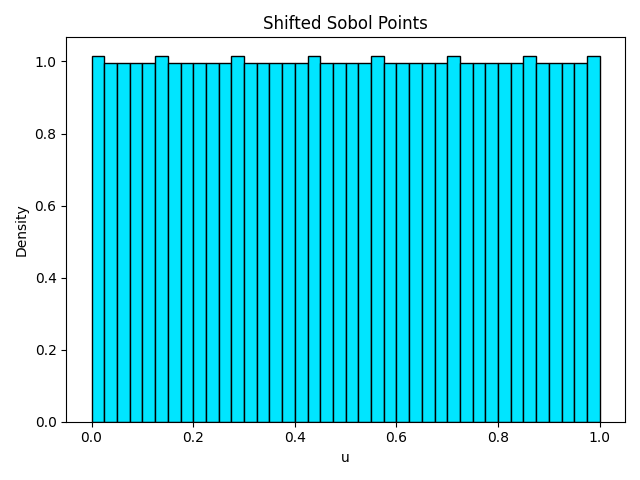
\includegraphics[width=\linewidth]{histogram1.png}
        \caption{}
        \label{shifted sobol}
    \end{subfigure}\hfill
    \begin{subfigure}{0.32\textwidth}
        \centering
        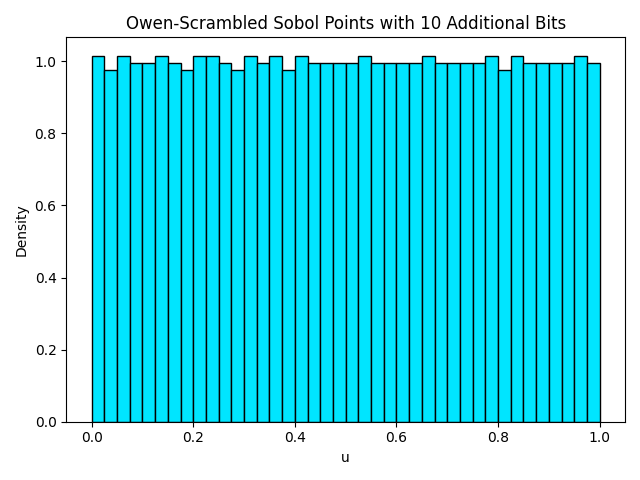
\includegraphics[width=\linewidth]{histogram2.png}
        \caption{}
        \label{scrambled sobol}
    \end{subfigure}\hfill
    \begin{subfigure}{0.32\textwidth}
        \centering
        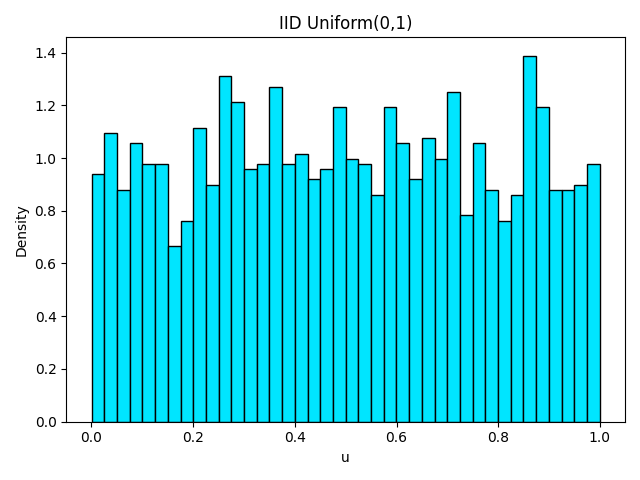
\includegraphics[width=\linewidth]{histogram3.png}
        \caption{}
        \label{drawn uniform}
    \end{subfigure}
    \caption{Histograms of Different Point Sets in the Interval $[0,1]$}
    \label{histograms}
\end{figure}
\subsubsection{Truncation Regions}
\noindent To choose our truncation region, we need to make sure that all the points that we use in the entropy estimate, are in the region where the function that we are integrating is not truncated so that for all the points that we are using we have $\hat{g}(u)=g(u)$ so that we are still integrating the same function but on a smaller region 
\begin{lemma}
\label{lem:r3}
 Let $\mathcal{P}_{\text{shifted}}$ be as Theorem~\ref{th:r5}, then $\forall\;x\in\mathcal{P}_{\text{shifted}}\;, x \in\Bigl[\frac{1}{2n},1-\frac{1}{2n}\Bigr]$ 
 \end{lemma}
\begin{proof}
The upper limit is established in the proof of theorem \ref{th:r5}. For the lower limit , we have $x_i+\delta_i\geq 0 +\frac{1}{2n}=\frac{1}{2n}$
\end{proof}
\noindent Let $\mathcal{P}_{\text{scrambled}}$ be the same as in Theorem \ref{thm: approximate scrambling}, by Lemma \label{lem:r1} in \ref{app: Owen Scrambling}, we have that $\forall x\in\mathcal{P}_{\text{scrambled}},x\in\left[\frac{1}{2^k n},1-\frac{1}{2^k n}\right]$. Therefore, for each case the truncation regions are given by 
\begin{equation}
\label{eq:gghat}
\hat{g}_{\text{shifted}}(u)=\begin{cases} g(u) & \text{ if } u \in \left[\frac{1}{2n} , 1-\frac{1}{2n}\right]\\
0 & \text{ otherwise }
    \end{cases}\qquad 
\hat{g}_{\text{scrambled}}(u)=\begin{cases} g(u) & \text{ if } u \in \left[\frac{1}{2^{k}n} , 1-\frac{1}{2^{k}n}\right]\\
0 & \text{ otherwise }
    \end{cases}
\end{equation}

\section{Error Analysis of QMC and RQMC Entropy Estimates}
In this section, we obtain the complexity of the error of the QMC and RQMC entropy estimates.We first start with the RQMC method.
\subsection{Error From RQMC Estimate}
In this section   let $\mathcal{P}_{\text{scr}}=\{u_1,u_2,\ldots,u_n\}$ be the same as in Theorem \ref{thm: approximate scrambling} and let $X$ be a normalized alpha stable RV $X\sim\mathbf{S}(\alpha,\beta;0)$ with PDF $f(x|\alpha,\beta;k)=f(x)$ and CDF $F(x)$, and let $h(X)$ be the true value of the differential entropy and consider the RQMC entropy estimate \begin{equation}
    h_m=\frac{1}{2^m}\sum_{u\in\mathcal{P}_{\text{scr}}}\hat{g}_{\text{scr}}(u) \qquad 
\hat{g}_{\text{scr}}(u)=\begin{cases} g(u) & \text{ if } u \in \left[\frac{1}{2^{k}n} , 1-\frac{1}{2^{k}n}\right]\\
0 & \text{ otherwise }
    \end{cases}
\qquad g(u) \triangleq -\log(f(F^{-1}(u)))
\end{equation} 
where $n=2^m$, and we analyze the complexity in terms of $m$ because for Theorem $\ref{thm: approximate scrambling}$ to hold, we need the point set before approximated scrambling to be a $(t,m,1)$ net , so $n$ has to be a power of 2 and writing $n\to\infty$ does not in general mean that $n$ is increasing in powers of 2. 
\begin{lemma}
\label{lem: general error}The absolute error \(\lvert h-h_m\rvert\) satisfies  \(\lvert h-h_m\rvert\leq\delta_{m,1} + \delta_{m,2}\) where \begin{equation}\label{deltaN1}
\delta_{m,1}\triangleq \left\lvert \int_0^1g(u)du-\int_0^1\hat{g}_{\text{scr}}(u)du\right\rvert
\end{equation}
\begin{equation}
\label{deltaN2}
\delta_{m,2}\triangleq\left\lvert \int_0^1\hat{g}_{\text{scr}}(u)du-\frac{1}{2^m}\sum_{u\in\mathcal{P}_{\text{scr}}}\hat{g}_{\text{scr}}(u)\right\rvert
\end{equation}
\end{lemma}
\begin{proof}
\begin{align*}
 \lvert h-h_m\rvert
 &=\left\lvert \int_0^1g(u)du-\frac{1}{2^m}\sum_{u\in\mathcal{P}_{\text{scr}}}\hat{g}_{\text{scr}}(u)\right\rvert\\
&\leq \left\lvert \int_0^1g(u)du-\int_0^1\hat{g}_{\text{scr}}(u)du\right\rvert+ \left\lvert \int_0^1\hat{g}_{\text{scr}}(u)du-\frac{1}{2^m}\sum_{u\in\mathcal{P}_{\text{scr}}}\hat{g}_{\text{scr}}(u)\right\rvert \\
&= \delta_{m,1} + \delta_{m,2}
\end{align*}
\end{proof}
\noindent In what follows, we analyze the behavior of each of the two error terms as a function of $m$ under certain assumptions. 
\begin{lemma}
\label{lem:del1}Let $\delta_{m,1}$ be the same as in \eqref{deltaN1} and assume that $\alpha\neq2$ and $\lvert \beta\rvert \neq 1$ then $\delta_{m,1}\in\mathcal{O}\left(\frac{m}{2^m}\right)\;\;\;m\to\infty$\end{lemma}

\begin{proof}
\begin{align*}
\delta_{m,1}&= \left\lvert \int_0^1g(u)du-\int_0^1\hat{g}_{\text{scr}}(u)du\right\rvert
=\left\lvert \int_0^1g(u)du-\int_{\frac{1}{2^{m+k}}}^{1-\frac{1}{2^{m+k}}} g(u)du\right\rvert=\left\lvert \int_{0}^{\frac{1}{2^{m+k}}}g(u)du+\int_{1-\frac{1}{2^{m+k}}}^{1}g(u)du\right\rvert \\
&\leq \left\lvert \int_{0}^{\frac{1}{2^{m+k}}}g(u)du\right\rvert +\left\lvert \int_{1-\frac{1}{2^{m+k}}}^{1}g(u)du\right\rvert
\end{align*}
Now let \begin{equation}
    I=\left\lvert \int_{0}^{\frac{1}{2^{m+k}}}g(u)du\right\rvert \qquad   \text{ and } \qquad J=\left\lvert \int_{1-\frac{1}{2^{m+k}}}^{1}g(u)du\right\rvert.
\end{equation} 
\noindent Replacing $g(u) \triangleq -\log(f(F^{-1}(u)))$, we get 

\begin{equation}
    I=\left\lvert -\int_{-\infty}^{F^{-1}\left(\frac{1}{2^{m+k}}\right)}f(x)\log f(x)dx\right\rvert \qquad   \text{ and } \qquad J=\left\lvert - \int_{F^{-1}\left({1-\frac{1}{2^{m+k}}}\right)}^{\infty}f(x)\log f(x)dx\right\rvert
\end{equation} 
In order to find a tight upper bound for  $I$, we use the tail approximation property present in  \eqref{pr:tail-approximation} which implies that $\forall\; \epsilon >0 ,\exists \;M < 0$ such that \begin{equation}
    \left\lvert \frac{f(x)}{\alpha C_\alpha (1-\beta) (-x)^{-(\alpha+1)}}-1 \right\rvert <\epsilon \qquad \forall x\leq  M 
\end{equation}
Let $k(\alpha,\beta)=\alpha C_\alpha (1-\beta)$ and let $\epsilon =\frac{1}{2}$ then $\exists \; M_1 < 0$ such that \begin{equation}
    \left\lvert \frac{f(x)}{k(\alpha,\beta) (-x)^{-(\alpha+1)}}-1 \right\rvert <\frac{1}{2} \Rightarrow \frac{1}{2}k(\alpha,\beta) (-x)^{-(\alpha+1)} < f(x) < \frac{3}{2}k(\alpha,\beta) (-x)^{-(\alpha+1)}
\end{equation}
Choose $m$ large enough so that $F^{-1} \left(\frac{1}{2^{m+k}}\right) < M_1$ then
\begin{align*}
I&=\left\lvert -\int_{-\infty}^{F^{-1}\left(\frac{1}{2^{m+k}}\right)}f(x)\log f(x)dx\right\rvert=\int_{-\infty}^{F^{-1}\left(\frac{1}{2^{m+k}}\right)}- f(x)\log f(x)dx\\
&\leq \int_{-\infty}^{F^{-1}\left(\frac{1}{2^{m+k}}\right)} - \frac{1}{2}k(\alpha,\beta) (-x)^{-(\alpha+1)} \log \left[\frac{3}{2}k(\alpha,\beta) (-x)^{-(\alpha+1)}\right] dx \\
&\leq (\alpha+1)\frac{1}{2}k(\alpha,\beta) \int_{-F^{-1}\left(\frac{1}{2^{m+k}}\right)}^{\infty}  t^{-(\alpha+1)} \log \Bigl[ \ell(\alpha,\beta) t\Bigl] dt,
\end{align*}
where $t = -x$ and $\ell(\alpha,\beta)=\left(\frac{3}{2}k(\alpha,\beta)\right)^{-\frac{1}{1+\alpha }}$. Let 
\(u=\log\Bigl[\ell(\alpha,\beta)t\Bigr]\), we obtain 

 \begin{equation}\label{eq:bound for I}
I\leq(\alpha+1)\frac{1}{2}k(\alpha,\beta)\ell(\alpha,\beta)^{\alpha} \int_{\log\Bigr[-\ell(\alpha,\beta) F^{-1}\left(\frac{1}{2^{m+k}}\right)\Bigr]}^{\infty } ue^{-\alpha u} du = (\alpha+1)\frac{1}{2}k(\alpha,\beta)\ell(\alpha,\beta)^{\alpha} A
\end{equation}

where \begin{equation}
    A\triangleq \int_{\log\Bigr[-\ell(\alpha,\beta)
F^{-1}(\tfrac{1}{2^{m+k}})\Bigr]}^{\infty }
u e^{-\alpha u}\,du
\end{equation} Using Integration by parts, we get that \begin{equation}\label{eq:Iintergal}
A= \log\Bigr[-\ell(\alpha,\beta)
F^{-1}\!\left(\tfrac{1}{2^{m+k}}\right)\Bigr]
\Biggr[\left(-\ell(\alpha,\beta)
F^{-1}\!\left(\tfrac{1}{2^{m+k}}\right)\right)^{-\alpha}\Biggr] \\
 +\frac{1}{\alpha^2}
 \Biggr[\left(-\ell(\alpha,\beta)
F^{-1}\!\left(\tfrac{1}{2^{m+k}}\right)\right)^{-\alpha}\Biggr]    
\end{equation}
 Using Nolan's assymptotic for tail probabilities \cite{NolanJohnP2020USDM}.
 \begin{equation}
     \mathbb{P}(X<-x)\sim  C_{\alpha}(1-\beta)x^{-\alpha}  \qquad \text{ as } x\to\infty\end{equation} 
then $\forall \; \epsilon >0\;  \exists\; M$ such that \begin{equation}
    \left\lvert \frac{F(-x)}{ C_{\alpha}(1-\beta)x^{-\alpha}}-1\right\rvert <\epsilon\qquad \forall x>M
\end{equation} 
Let $\epsilon=\frac{1}{2^{k}}$ then $\exists \; M_2$ such that 
\begin{equation}
    \left\lvert \frac{F(-x)}{ C_{\alpha}(1-\beta)x^{-\alpha}}-1\right\rvert <\frac{1}{2^{k} }\qquad \forall x>M_2 
\end{equation}
\begin{equation}
    \frac{2^{k}-1}{2^{k}} C_{\alpha}(1-\beta)x^{-\alpha}<  F(-x)\ <\frac{2^{k}+1}{2^{k} } C_{\alpha}(1-\beta)x^{-\alpha}\qquad \forall x>M_2
\end{equation} 
Since the CDF is increasing we obtain $\forall x>M_2$
\begin{equation}
F^{-1}\left(\frac{2^{k}-1}{2^{k}} C_{\alpha}(1-\beta)x^{-\alpha}\right) \leq 
-x \leq F^{-1}\left( \frac{2^{k}+1}{2^{k} }C_{\alpha}(1-\beta)x^{-\alpha}\right) \label{eq:star}
\end{equation}
Choose $m$ large enough so that \begin{equation}
    2^m \geq \frac{M_2^{\alpha}}{(2^{k}-1)C_{\alpha}(1-\beta)}
\Rightarrow ((2^{k}-1)C_{\alpha}(1-\beta)2^m)^{\frac{1}{\alpha}} \geq M_2
\end{equation} 
Therefore, equation~\eqref{eq:star} implies for $x = ((2^{k}-1)C_{\alpha}(1-\beta)2^m)^{\frac{1}{\alpha}}$
\begin{equation}
    F^{-1}\left(\frac{1}{2^{m+k}}\right)  \leq  -((2^{k}-1)C_{\alpha}(1-\beta)2^m)^{\frac{1}{\alpha}}\\ \leq F^{-1}\left( \frac{2^{k}+1}{2^{k}(2^{k}-1)2^m}\right)
\end{equation}
which gives  
\begin{equation}
\left(-\ell(\alpha,\beta)F^{-1}\left(\frac{1}{2^{m+k}}\right)\right)^{-\alpha} \leq \left( \ell(\alpha,\beta)((2^{k}-1)C_{\alpha}(1-\beta)2^m)^{\frac{1}{\alpha}}\right)^{-\alpha} \label{eq:starstar}
\end{equation}
Similarly, choosing $m$ large enough so that \( 2^m \geq \frac{M_2^{\alpha}}{(2^{k}+1)C_{\alpha}(1-\beta)}\)
\begin{equation}
\ell(\alpha,\beta)((2^{k}+1)C_{\alpha}(1-\beta)2^m)^{\frac{1}{\alpha}} \geq  -\ell(\alpha,\beta)F^{-1}\left( \frac{1}{2^{m+k}}\right) 
\label{eq:starstarstar}
\end{equation}
Returning to equation \eqref{eq:Iintergal}, we write
\begin{align}
&A = \log\Bigr[-\ell(\alpha,\beta) F^{-1}\left(\frac{1}{2^{m+k}}\right)\Bigr] \left(-\ell(\alpha,\beta) F^{-1}\left(\frac{1}{2^{m+k}}\right)\right)^{-\alpha}\nonumber\\&\qquad \qquad \qquad \qquad + \frac{1}{\alpha^2}\left(-\ell(\alpha,\beta) F^{-1}\left(\frac{1}{2^{m+k}}\right)\right)^{-\alpha}\nonumber\\
&\leq \log\Big[\ell(\alpha,\beta)((2^{k}+1)C_{\alpha}(1-\beta))^{\frac{1}{\alpha}}2^{\frac{m}{\alpha}})\Bigr]\frac{ ((2^{k}-1)C_{\alpha}(1-\beta))^{-1}\ell(\alpha,\beta)^{-\alpha}}{2^m}\nonumber\\
&\qquad \qquad \qquad \qquad +\frac{1}{\alpha^2}\frac{ (C_{\alpha}(1-\beta)(2^{k}-1))^{-1}\ell(\alpha,\beta)^{-\alpha}}{2^m} \label{eq:usestars}\\
&\in \mathcal{O}\left(m\right) \times \mathcal{O}\left(\frac{1}{2^m}\right)+\mathcal{O}\left(\frac{1}{2^m}\right) \nonumber\\
& \in\mathcal{O}\left(\frac{m}{2^m}\right)\;\;\; m\to\infty \label{eq:comp1},
\end{align}
where we used equations~\eqref{eq:starstar} and~\eqref{eq:starstarstar} in order to write equation~\eqref{eq:usestars}. Since $I 
\leq (\alpha+1)\frac{1}{2}k(\alpha,\beta)\ell(\alpha,\beta)^{\alpha} A$ (equation~\eqref{eq:bound for I}), then equation~\eqref{eq:comp1} implies that 
\begin{equation}
\label{eq:comp2}
I \in \mathcal{O}\left(\frac{m}{2^m}\right)\;\;\;m\to\infty.
\end{equation}
We can follow similar steps for $J$, and we get that 
\begin{equation}
J \in \mathcal{O}\left(\frac{m}{2^m}\right)\;\;\;m\to\infty 
\label{eq:comp3}
\end{equation}
Finally 
\begin{equation}
\delta_{m,1} \leq I+J\in\mathcal{O}\left(\frac{m}{2^m}\right)\;\;\;m\to\infty
\label{eq:comp4} 
\end{equation}
\end{proof}
\begin{lemma}
\label{lem:e3}Let $
 \delta_{m,2}$ be the same as in \eqref{deltaN2}, and assume that our stable RV does not have the parameters $\alpha=2$ ,$(\alpha=1,\beta\neq0)$, and  $\lvert \beta\rvert\neq1$ then $\delta_{m,2} \in\mathcal{O}\left( \frac{m}{2^m}\right)\;\;\;m\to\infty$
 \end{lemma}
\begin{proof}
\begin{equation}
\label{using upper bound}
\delta_{m,2}=\left\lvert \int_0^1\hat{g}_{\text{scr}}(u)du-\frac{1}{2^m}\sum_{u\in\mathcal{P}_{\text{scr}}}\hat{g}_{\text{scr}}(u)\right\rvert
\leq V(\hat{g}_{\text{scr}})D^{\ast}_{2^m}(\mathcal{P}_{\text{scr}}),
\end{equation}
where we applied Theorem \ref{th:KH} to write the upperbound, and Theorem \ref{th:KH} applies because the variation in the sense of Hardy and Krause for $\hat{g}_{\text{scr}}(u)$ is a finite integral.Since our stable RV does not have the parameters $\alpha=2$,$(\alpha=1,\beta\neq0)$, and  $\lvert\beta\rvert\neq1$, we can use the asymptotic properties of the derivative of the pdf of our stable RV.We will use the fact that under these assumptions on $\alpha$ and $\beta$, we have \(f^{\prime}(x)=\mathcal{O}\left(\frac{1}{\lvert x\rvert ^{\alpha+2}}\right)\) as $\lvert x\rvert\to\infty$ which is proven in \cite{alma991006837049709436}.Using this asymptotic and using Nolan's tail approximation we get that $\exists \;T>0$ such that  
\begin{eqnarray}
f(x) &>& \frac{1}{2}k(\alpha,\beta) |x|^{-(\alpha+1)} \label{eq:pdfapp}\\
\lvert f^{\prime}(x)\rvert &\leq& \frac{L}{\lvert x \rvert ^{\alpha +2}}, \label{eq:derapp}
\end{eqnarray}
for some $L > 0$ and for all $|x| \geq T$, and where $k(\alpha,\beta)$ has been previously defined. 
Let $m > 0$ be large enough, so that $F^{-1}\left(\frac{1}{2^{m+k}}\right) \leq  -T$ and $F^{-1}\left(1-\frac{1}{2^{m+k}}\right) \geq T$, then 
\begin{align*} 
V(\hat{g}_{\text{scr}})&= \int_{F^{-1}\left(\frac{1}{2^{m+k}}\right)}^{F^{-1}\left(1-\frac{1}{2^{m+k}}\right)}\left\lvert \frac{f^{\prime}(x)}{f(x)}\right\rvert dx \\
&=\int_{{F^{-1}\left(\frac{1}{2^{m+k}}\right)}}^{-T}\left\lvert \frac{f^{\prime}(x)}{f(x)} \right\rvert dx+ \int_{-T}^{T} \left\lvert \frac{f^{\prime}(x)}{f(x)} \right\rvert dx + \int_{T}^{F^{-1}\left(1-\frac{1}{2^{m+k}}\right)}\left\lvert \frac{f^{\prime}(x)}{f(x)} \right\rvert dx.
\end{align*}
Using equations~\eqref{eq:pdfapp} and~\eqref{eq:derapp}, we get 
\begin{align*}
\int_{{F^{-1}\left(\frac{1}{2^{m+k}}\right)}}^{-T}\left\lvert \frac{f^{\prime}(x)}{f(x)} \right\rvert dx &\leq
\frac{2L}{k(\alpha,\beta) }\int_{T}^{-{F^{-1}(\frac{1}{2^{m+k}})}}\frac{1}{t} dt\\
&=\frac{2L}{k(\alpha,\beta)}\left(\log\left(-{F^{-1}\left(\frac{1}{2^{m+k}}\right)}\right)-\log(T)\right)\\
&\in \mathcal{O}\left(m\right),
\end{align*}
where we used the fact that $
    -{F^{-1}\left(\frac{1}{2^{m+k}}\right)} \in \mathcal{O}\left(2^{\frac{m}{\alpha}}\right)
$ as shown in Lemma~\ref{lem:del1}.  
Similarly, one can show
\begin{equation}
\int_{T}^{ {F^{-1}(1-\frac{1}{2^{m+k}})}} \left\lvert \frac{f^{\prime}(x)}{f(x)} \right\rvert dx \in\mathcal{O}\left(m\right)\;\;\;m\to\infty,
\end{equation}
Therefore, 
\begin{align*} 
V(\hat{g}_{\text{scr}})&= \int_{F^{-1}(\frac{1}{2^{m+k}})}^{F^{-1}(1-\frac{1}{2^{m+k}})}\left\lvert \frac{f^{\prime}(x)}{f(x)}\right\rvert dx \\
&=\int_{{F^{-1}\left(\frac{1}{2^{m+k}}\right)}}^{-T}\left\lvert \frac{f^{\prime}(x)}{f(x)} \right\rvert dx+ \int_{-T}^{T} \left\lvert \frac{f^{\prime}(x)}{f(x)} \right\rvert dx + \int_{T}^{F^{-1}\left(1-\frac{1}{2^{m+k}}\right)}\left\lvert \frac{f^{'}(x)}{f(x)} \right\rvert dx
\end{align*}
Both tail integrals grow as $\mathcal{O}(m)\;\;\;m\to\infty$ and the body integral is a constant therefore \begin{equation}
    V(\hat{g}_{\text{scr}})\in\mathcal{O}(m)\;\;\;m\to\infty
\end{equation}
Finally, 
\begin{align*} 
\delta_{m,2}&\leq V(\hat{g}_{\text{scr}})D^{\ast}_{2^m}(\mathcal{P}_{\text{scr}}) && \text{\eqref{using upper bound}}\\
&\in \mathcal{O}(m)D^{\ast}_{2^m}(\mathcal{P}_{\text{scr}})\\
&\leq \mathcal{O}(m)\frac{1+2^{t}}{2^{m}} && \text{ (Theorem \ref{thm: approximate scrambling}) }\\
&\in\mathcal{O}(m)\mathcal{O}\left(\frac{1}{2^m}\right)\in\mathcal{O}\left(\frac{m}{2^m}\right)\;\;\;m\to\infty
\end{align*}
\end{proof}
\begin{theorem}
     Assume that the parameters of our stable RV are not $\alpha=2,(\alpha=1,\beta\neq0)$, and $\lvert \beta\rvert\neq 1$ then $\lvert h-h_m\rvert\in\mathcal{O}\left(\frac{m}{2^m}\right)\;\;\;m\to\infty$.

\end{theorem}
    \begin{proof}the result follows from  Lemmas \ref{lem: general error}, \ref{lem:del1}, and \ref{lem:e3}.
    \end{proof}
    \subsection{Error From QMC Estimate}
    In this section   let $\mathcal{P}_{\text{shift}}=\{u_1,u_2,\ldots,u_n\}$ be the same as in Theorem \ref{th:r5} and let $X$ be a normalized alpha stable RV $X\sim\mathbf{S}(\alpha,\beta;0)$ with PDF $f(x|\alpha,\beta;k)=f(x)$ and CDF $F(x)$, and let $h(X)$ be the true value of the differential entropy and consider the RQMC entropy estimate \begin{equation}
    h_m=\frac{1}{2^m}\sum_{u\in\mathcal{P}_{\text{shift}}}\hat{g}_{\text{shift}}(u) \qquad 
\hat{g}_{\text{shift}}(u)=\begin{cases} g(u) & \text{ if } u \in \left[\frac{1}{2n} , 1-\frac{1}{2n}\right]\\
0 & \text{ otherwise }
    \end{cases}
\qquad g(u) \triangleq -\log(f(F^{-1}(u)))
\end{equation}
\begin{theorem}
Assume that the parameters of our stable RV are not $\alpha=2,(\alpha=1,\beta\neq0)$, and $\lvert \beta\rvert\neq 1$ then $\lvert h-h_m\rvert\in\mathcal{O}\left(\frac{m}{2^m}\right)\;\;\;m\to\infty$.
\end{theorem}
    \begin{proof}
We can see that $g_{\text{shift}}(u)$ is the same as $g_{\text{scr}}(u)$ with $k=1$ therefore the same analysis for $g_{\text{scr}}(u)$ holds for $g_{\text{shift}}(u)$  in Lemma \ref{lem:del1}. Moreover, $\mathcal{P}_{\text{shift}}$ and $\mathcal{P}_{\text{scr}}$ share the same discrepancy bound as seen in inequalities \eqref{same bound two} and \eqref{same bound one} then the same analysis for $\mathcal{P}_{\text{scr}}$  holds for $\mathcal{P}_{\text{shift}}$ in Lemma \ref{lem:e3}  hence the result follows after expressing the  error in the same way as in Lemma \ref{lem: general error}.    
    \end{proof}
\section{The Cauchy Distribution}
We consider the standard Cauchy distribution, whose differential entropy is given by $h(X)=\log(4\pi)$\cite{NolanJohnP2020USDM}. We compute the entropy using classical MC simulation with 60 independent repetitions for each value of $n$ and the resulting estimate is the average value of the independent trials, the QMC method, and the RQMC method with 60 independent repetitions for each value of $n$ and we average over the independent trials as in the MC method, and we use 6 additional for the approximate Owen Scrambling.The resulting plot for the absolute error of the three computations is given in the following figure.
\begin{figure}[H]
    \centering
    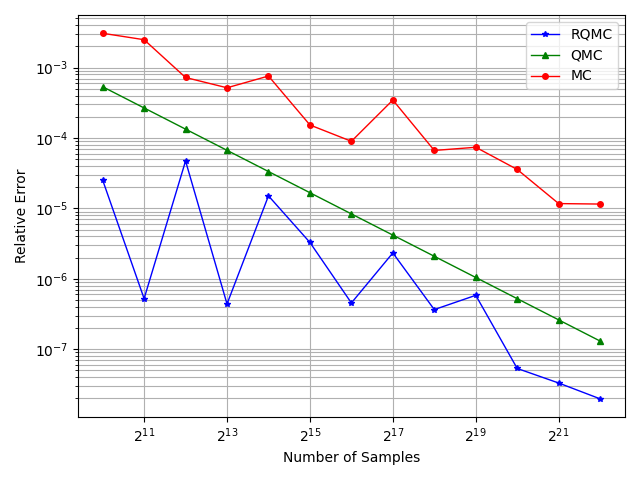
\includegraphics[height=0.33\textheight ,width=0.62\textwidth]{relative_errors.png}
    \caption{Relative Error Plots for MC,QMC, and RQMC methods}
    \label{rel error plot}
\end{figure}
\noindent We can see that the RQMC method generally performs better than the QMC method; however, the RQMC method takes more time due to several independent trials.We can also see that both methods perform better than the classical MC simulation method.
\newpage
\section{Table of Differential Entropy Values for Stable Distributions}
\begin{table}[ht]
\centering
\begin{tabular}{cccccccccccc}
\toprule
\(\beta\) & 0.0 & 0.1 & 0.2 & 0.3 & 0.4 & 0.5 & 0.6 & 0.7 & 0.8 & 0.9 & 1.0 \\
\(\alpha\) &  &  &  &  &  &  &  &  &  &  &  \\
\midrule
0.40 & 4.121\textcolor{red}{0} & 4.118\textcolor{red}{8} & 4.111\textcolor{red}{9} & 4.1001 & 4.0831 & 4.0603 & 4.0307 & 3.9925 & 3.9430 & 3.8755 & 3.7577 \\
0.45 & 3.8579 & 3.8558 & 3.8494 & 3.8385 & 3.8228 & 3.8016 & 3.7741 & 3.7386 & 3.6926 & 3.6297 & 3.5196 \\
0.50 & 3.6399 & 3.6380 & 3.6320 & 3.6219 & 3.6073 & 3.5876 & 3.5619 & 3.5290 & 3.4860 & 3.4273 & 3.3245 \\
0.55 & 3.4558 & 3.4539 & 3.4484 & 3.4389 & 3.4253 & 3.4069 & 3.3830 & 3.3523 & 3.3122 & 3.2574 & 3.1613 \\
0.60 & 3.2976 & 3.2959 & 3.2907 & 3.2819 & 3.2692 & 3.2520 & 3.2297 & 3.2009 & 3.1635 & 3.1122 & 3.0225 \\
0.65 & 3.1600 & 3.1584 & 3.1536 & 3.1453 & 3.1334 & 3.1174 & 3.0965 & 3.0696 & 3.0345 & 2.9866 & 2.9029 \\
0.70 & 3.0389 & 3.0375 & 3.0329 & 3.0252 & 3.0140 & 2.9990 & 2.9795 & 2.9543 & 2.9215 & 2.8767 & 2.7986 \\
0.75 & 2.9314 & 2.9300 & 2.9258 & 2.9185 & 2.9081 & 2.8940 & 2.8757 & 2.8521 & 2.8214 & 2.7795 & 2.7068 \\
0.80 & 2.8347 & 2.8335 & 2.8295 & 2.8228 & 2.8131 & 2.7999 & 2.7827 & 2.7607 & 2.7319 & 2.6928 & 2.6252 \\
0.85 & 2.7471 & 2.7460 & 2.7424 & 2.7361 & 2.7270 & 2.7147 & 2.6986 & 2.6780 & 2.6511 & 2.6145 & 2.5517 \\
0.90 & -- & -- & 2.6633 & -- & -- & -- & -- & -- & -- & 2.5438 & 2.4855 \\
0.95 & 2.5933 & -- & 2.5904 & 2.5850 & 2.5770 & 2.5662 & 2.5522 & 2.5341 & 2.5106 & 2.4788 & 2.4249 \\
1.00 & 2.5310 & -- & -- & -- & -- & -- & -- & -- & -- & -- & -- \\
1.05 & 2.4699 & 2.4690 & 2.4661 & 2.4612 & 2.4542 & 2.4445 & 2.4321 & 2.4163 & 2.3958 & 2.3683 & 2.3225 \\
1.10 & 2.4133 & 2.4124 & 2.4098 & 2.4052 & 2.3986 & 2.3898 & 2.3783 & 2.3636 & 2.3447 & 2.3192 & 2.2772 \\
1.15 & 2.3606 & 2.3598 & 2.3573 & 2.3530 & 2.3469 & 2.3387 & 2.3280 & 2.3144 & 2.2969 & 2.2734 & 2.2350 \\
1.20 & 2.3114 & 2.3106 & 2.3083 & 2.3043 & 2.2987 & 2.2910 & 2.2811 & 2.2685 & 2.2523 & 2.2307 & 2.1958 \\
1.25 & 2.2652 & 2.2645 & 2.2623 & 2.2587 & 2.2534 & 2.2464 & 2.2372 & 2.2256 & 2.2107 & 2.1909 & 2.1593 \\
1.30 & 2.2217 & 2.2211 & 2.2191 & 2.2157 & 2.2109 & 2.2044 & 2.1960 & 2.1853 & 2.1717 & 2.1536 & 2.1251 \\
1.35 & 2.1807 & 2.1801 & 2.1782 & 2.1752 & 2.1707 & 2.1648 & 2.1571 & 2.1474 & 2.1350 & 2.1186 & 2.0931 \\
1.40 & 2.1418 & 2.1412 & 2.1395 & 2.1367 & 2.1327 & 2.1273 & 2.1203 & 2.1115 & 2.1003 & 2.0856 & 2.0629 \\
1.45 & 2.1048 & 2.1043 & 2.1028 & 2.1002 & 2.0965 & 2.0917 & 2.0854 & 2.0775 & 2.0674 & 2.0543 & 2.0344 \\
1.50 & 2.0694 & 2.0690 & 2.0677 & 2.0654 & 2.0621 & 2.0577 & 2.0521 & 2.0451 & 2.0362 & 2.0246 & 2.0073 \\
1.55 & 2.0356 & 2.0353 & 2.0341 & 2.0320 & 2.0291 & 2.0253 & 2.0203 & 2.0141 & 2.0063 & 1.9963 & 1.9814 \\
1.60 & 2.0032 & 2.0028 & 2.0018 & 2.0000 & 1.9975 & 1.9941 & 1.9899 & 1.9845 & 1.9778 & 1.9692 & 1.9566 \\
1.65 & 1.9718 & 1.9715 & 1.9707 & 1.9691 & 1.9670 & 1.9641 & 1.9605 & 1.9559 & 1.9503 & 1.9431 & 1.9327 \\
1.70 & 1.9415 & 1.9412 & 1.9405 & 1.9392 & 1.9375 & 1.9351 & 1.9321 & 1.9283 & 1.9237 & 1.9178 & 1.9095 \\
1.75 & 1.9119 & 1.9117 & 1.9111 & 1.9101 & 1.9087 & 1.9068 & 1.9044 & 1.9014 & 1.8978 & 1.8932 & 1.8868 \\
1.80 & 1.8830 & 1.8829 & 1.8824 & 1.8816 & 1.8806 & 1.8791 & 1.8773 & 1.8751 & 1.8724 & 1.8689 & 1.8643 \\
1.85 & 1.8544 & 1.8543 & 1.8540 & 1.8535 & 1.8527 & 1.8518 & 1.8505 & 1.8490 & 1.8471 & 1.8448 & 1.8417 \\
1.90 & 1.8259 & 1.8259 & 1.8257 & 1.8254 & 1.8250 & 1.8244 & 1.8237 & 1.8228 & 1.8217 & 1.8204 & 1.8186 \\
1.95 & 1.7969 & 1.7969 & 1.7969 & 1.7967 & 1.7966 & 1.7963 & 1.7961 & 1.7957 & 1.7953 & 1.7948 & 1.7941 \\
2.00 & 1.7655 & 1.7655 & 1.7655 & 1.7655 & 1.7655 & 1.7655 & 1.7655 & 1.7655 & 1.7655 & 1.7655 & 1.7655 \\
\bottomrule
\end{tabular}

\caption{Estimated differential entropy of stable distributions as a function of 
\(\alpha\) and \(\beta\).}
\end{table}
\begin{table}[ht]
\centering
\begin{tabular}{cccccccccccc}
\toprule
$\beta$ & 0.0 & 0.1 & 0.2 & 0.3 & 0.4 & 0.5 & 0.6 & 0.7 & 0.8 & 0.9 & 1.0 \\
$\alpha$ &  &  &  &  &  &  &  &  &  &  &  \\
\midrule
0.40 & 4.1208 & 4.1185 & 4.1116 & 4.0998 & 4.0829 & 4.0601 & 4.0304 & 3.9923 & 3.9428 & 3.8753 & 3.7576 \\
0.45 & 3.8578 & 3.8557 & 3.8493 & 3.8384 & 3.8227 & 3.8015 & 3.7740 & 3.7385 & 3.6925 & 3.6296 & 3.5196 \\
0.50 & 3.6398 & 3.6379 & 3.6319 & 3.6218 & 3.6072 & 3.5875 & 3.5619 & 3.5289 & 3.4859 & 3.4273 & 3.3244 \\
0.55 & 3.4557 & 3.4538 & 3.4483 & 3.4388 & 3.4252 & 3.4068 & 3.3829 & 3.3521 & 3.3120 & 3.2572 & 3.1612 \\
0.60 & 3.2975 & 3.2958 & 3.2906 & 3.2818 & 3.2690 & 3.2519 & 3.2296 & 3.2008 & 3.1633 & 3.1121 & 3.0225 \\
0.65 & 3.1599 & 3.1583 & 3.1535 & 3.1451 & 3.1332 & 3.1172 & 3.0963 & 3.0694 & 3.0344 & 2.9865 & 2.9028 \\
0.70 & 3.0387 & 3.0372 & 3.0327 & 3.0249 & 3.0138 & 2.9988 & 2.9792 & 2.9540 & 2.9212 & 2.8764 & 2.7983 \\
0.75 & 2.9311 & 2.9297 & 2.9255 & 2.9182 & 2.9078 & 2.8937 & 2.8754 & 2.8518 & 2.8211 & 2.7793 & 2.7066 \\
0.80 & 2.8348 & 2.8335 & 2.8295 & 2.8227 & 2.8130 & 2.7998 & 2.7826 & 2.7605 & 2.7317 & 2.6926 & 2.6249 \\
0.85 & 2.7479 & 2.7467 & 2.7429 & 2.7366 & 2.7274 & 2.7150 & 2.6989 & 2.6783 & 2.6513 & 2.6147 & 2.5519 \\
0.90 & 2.6689 & 2.6677 & 2.6642 & 2.6582 & 2.6496 & 2.6380 & 2.6229 & 2.6036 & 2.5784 & 2.5442 & 2.4861 \\
0.95 & 2.5960 & 2.5949 & 2.5916 & 2.5860 & 2.5780 & 2.5671 & 2.5530 & 2.5348 & 2.5112 & 2.4792 & 2.4258 \\
1.00 & 2.5310 & 2.5297 & 2.5245 & 2.5184 & 2.5103 & 2.4999 & 2.4865 & 2.4695 & 2.4476 & 2.4184 & 2.3720 \\
1.05 & 2.4670 & 2.4660 & 2.4632 & 2.4583 & 2.4512 & 2.4418 & 2.4295 & 2.4138 & 2.3935 & 2.3663 & 2.3727 \\
1.10 & 2.4113 & 2.4104 & 2.4077 & 2.4032 & 2.3966 & 2.3878 & 2.3763 & 2.3617 & 2.3428 & 2.3175 & 2.2770 \\
1.15 & 2.3592 & 2.3584 & 2.3559 & 2.3517 & 2.3455 & 2.3373 & 2.3267 & 2.3131 & 2.2956 & 2.2722 & 2.2348 \\
1.20 & 2.3104 & 2.3096 & 2.3073 & 2.3034 & 2.2977 & 2.2901 & 2.2802 & 2.2676 & 2.2514 & 2.2299 & 2.1956 \\
1.25 & 2.2645 & 2.2638 & 2.2617 & 2.2580 & 2.2527 & 2.2457 & 2.2366 & 2.2250 & 2.2101 & 2.1903 & 2.1591 \\
1.30 & 2.2213 & 2.2206 & 2.2186 & 2.2152 & 2.2104 & 2.2039 & 2.1955 & 2.1849 & 2.1712 & 2.1532 & 2.1250 \\
1.35 & 2.1803 & 2.1797 & 2.1779 & 2.1748 & 2.1704 & 2.1644 & 2.1568 & 2.1470 & 2.1346 & 2.1183 & 2.0930 \\
1.40 & 2.1415 & 2.1410 & 2.1393 & 2.1365 & 2.1324 & 2.1270 & 2.1201 & 2.1113 & 2.1000 & 2.0854 & 2.0628 \\
1.45 & 2.1046 & 2.1041 & 2.1026 & 2.1000 & 2.0964 & 2.0915 & 2.0852 & 2.0773 & 2.0672 & 2.0541 & 2.0343 \\
1.50 & 2.0693 & 2.0689 & 2.0675 & 2.0653 & 2.0620 & 2.0576 & 2.0520 & 2.0450 & 2.0360 & 2.0245 & 2.0072 \\
1.55 & 2.0356 & 2.0352 & 2.0340 & 2.0319 & 2.0291 & 2.0252 & 2.0203 & 2.0141 & 2.0063 & 1.9962 & 1.9814 \\
1.60 & 2.0031 & 2.0028 & 2.0017 & 2.0000 & 1.9974 & 1.9941 & 1.9898 & 1.9844 & 1.9777 & 1.9691 & 1.9566 \\
1.65 & 1.9718 & 1.9715 & 1.9706 & 1.9691 & 1.9670 & 1.9641 & 1.9605 & 1.9559 & 1.9502 & 1.9430 & 1.9327 \\
1.70 & 1.9415 & 1.9412 & 1.9405 & 1.9392 & 1.9374 & 1.9351 & 1.9320 & 1.9283 & 1.9236 & 1.9178 & 1.9095 \\
1.75 & 1.9119 & 1.9117 & 1.9111 & 1.9101 & 1.9087 & 1.9068 & 1.9044 & 1.9014 & 1.8977 & 1.8931 & 1.8867 \\
1.80 & 1.8830 & 1.8828 & 1.8824 & 1.8816 & 1.8805 & 1.8791 & 1.8773 & 1.8751 & 1.8723 & 1.8689 & 1.8643 \\
1.85 & 1.8544 & 1.8543 & 1.8540 & 1.8535 & 1.8527 & 1.8517 & 1.8505 & 1.8490 & 1.8471 & 1.8448 & 1.8417 \\
1.90 & 1.8259 & 1.8259 & 1.8257 & 1.8254 & 1.8249 & 1.8243 & 1.8236 & 1.8227 & 1.8217 & 1.8203 & 1.8186 \\
1.95 & 1.7969 & 1.7969 & 1.7968 & 1.7967 & 1.7965 & 1.7963 & 1.7960 & 1.7957 & 1.7953 & 1.7947 & 1.7941 \\
2.00 & 1.7655 & 1.7655 & 1.7655 & 1.7655 & 1.7655 & 1.7655 & 1.7655 & 1.7655 & 1.7655 & 1.7655 & 1.7655 \\
\bottomrule
\end{tabular}

\caption{Estimated differential entropy of stable distributions as a function of 
\(\alpha\) and \(\beta\).}
\end{table}


\clearpage
\bibliographystyle{plain}  % or alpha, abbrv, etc.
\bibliography{ref} % without .bib extension
\clearpage
\begin{appendices}
 \section{Sobol Sequences}
 \label{app:sobol}
 In this appendix, we present an algorithm to generate Sobol Sequences which is taken from \cite{DickJosef2010D}. \\
 Let $p_1,\ldots,p_s\in \mathbb{F}_2[x]$ be primitive polynomials ordered according to their degree and let \begin{equation}
     p_i(x)=x^{e_i}+a_{1,i}x^{e_i-1}+a_{2,i}x^{e_i-2}+\cdot\cdot\cdot+ a_{e_i-1}x+1\qquad \text{ for } 1\leq i\leq s
 \end{equation}
  choose odd natrual numbers $1\leq m_{1,i},\cdot\cdot\cdot,m_{e_i,i}$ such that $m_{k,i}<2^k$ for $1\leq k\leq e_i$, and for all $k>e_i$ define $m_{k,i}$ recursively by \begin{equation}
      m_{k,i}=2a_{1,i}m_{k-1,i}\oplus\cdot\cdot\cdot\oplus 2^{e_i-1}a_{e_{i}-1}m_{k-e_i+1,i}\oplus2^{e_i}m_{k-e_i,i}\oplus m_{k-e_i,i}
  \end{equation} where $\oplus$ is the bit-by-bit exclusive or operator . The numbers \(v_{k,i}=\frac{m_{k,i}}{2^k}\) are called direction numbers. Then for $n=0,1,2,\cdot\cdot\cdot$ with base 2 expansion \(n=n_0+2n_1+\cdot\cdot\cdot 2^{r-1}n_{r-1}\) we define \begin{equation}\label{sobol formula}
      x_{n,i}=n_0v_{1.i}\oplus n_1v_{2.i}\oplus\cdot\cdot\cdot\oplus n_{r-1}v_{r,i}
  \end{equation}The Sobol' sequence is then the sequence of points $\mathbf{x}_0,\mathbf{x}_1,\cdot\cdot\cdot$ where $\mathbf{x}_n=(x_{n,1},x_{n,2},\cdot\cdot\cdot ,x_{n,s})$. For different components of the vector, the choices of $m$ and the polynomials have to be different. For more details on generating Sobol Sequences, we refer the reader to \cite{BratleyPaul1988A6IS}.\\
 \noindent\textbf{Example A.1.1:} Lets apply the algorithm described above to generate the first few points of the Sobol Sequence. \\
Let $e_1=3$ $a_1=0$ and $a_2=1$ so our primitive polynomial is \(p(x)=x^{3}+x+1\). We can pick \(m[1]=1\), \(m[2]=3\), and \(m[3]=7\). Then \begin{equation}
m[4]=2a_1m[3]\oplus 2^2a_2m[2]\oplus2^{3}m[1]\oplus m[1]=0\oplus12\oplus8\oplus1 =(0000)_2\oplus(1100)_2\oplus(1000)_2\oplus(0001)_2=(0101)_2=5
\end{equation}
similarly, \(m[5]=7\).Now we compute the direction numbers, and the resulting Sobol points using equation \eqref{sobol formula}. The results are shown in Table \ref{direction numbers} and Table \ref{Sobol Points}. 
\begin{table}[H]
\centering

\begin{minipage}{0.48\textwidth}
\centering
\begin{tabular}{|c|c|c|c|}
\hline
$n$ & $m[n]$ & $v[n] = \dfrac{m[n]}{2^n}$ & $v[n]$ in binary \\[5pt] \hline
1 & 1 & $0.5$     & $(0.1)_2$ \\ \hline
2 & 3 & $0.75$    & $(0.11)_2$ \\ \hline
3 & 7 & $0.875$   & $(0.111)_2$ \\ \hline
4 & 5 & $0.3125$  & $(0.0101)_2$ \\ \hline
5 & 7 & $0.21875$ & $(0.00111)_2$ \\ \hline
\end{tabular}
\caption{Values of $v[n]$}
\label{direction numbers}
\end{minipage}
\hfill
\begin{minipage}{0.48\textwidth}
\centering
\begin{tabular}{|c|c|c|c|}
\hline
$i$ & $i$ in binary  & expression of $z_i$ & $z_i$ \\ \hline
0 & $(0000)_2$ & $i_k v_k = 0 \;\forall k\Rightarrow z_i=0$ & $0$ \\ \hline
1 & $(0001)_2$ & $z_1=i_1 v_1 = v_1$&0.5 \\ \hline
2 & $(0010)_2$ & $z_2=i_2 v_2 = v_2$&0.75 \\ \hline
3 & $(0011)_2$ & $z_3=i_1v_1\oplus i_2v_2 $ & $0.25$ \\ \hline
4 & $(0100)_2$ & $z_4=i_3 v_3 = v_3$ & $0.875$ \\ \hline
5 & $(0101)_2$ & $z_5=i_1v_1\oplus i_3 v_3$ & $0.375$ \\ \hline
\end{tabular}
\caption{The first six points of the Sobol Sequence}
\label{Sobol Points}
\end{minipage}
\end{table}

\noindent\textbf{ Example A.1.2 :}
In this example, we verify that the first 8 points of the Sobol Sequence in $\mathbb{R}^2$ form a $(0,3,2)$ net in base 2.Consider the following set $\mathcal{P}$ of points in $\mathbb{R}^2$ which contains the first 8 points of the Sobol Sequence.That is, \(\mathcal{P}=\left\{(0,0), (0.5,0.5),(0.375,0.375),(0.125,0.625)(0.625,0.125),(0.75,0.25),(0.25,0.75,),(0.875,0.875)\right\}\).We have to consider all elementary intervals of area \(2^{0-3}=0.125\).Since \( s=2\), our elementary intervals have the form \(E=\prod_{i=1}^2[a_ib^{-d_i},(a_i+1)b^{-d_i})\).The length of the first side is \(L_1=(a_1+1)2^{-d_1} - (a_1)2^{-d_1}=2^{-d_1}\), and the length of the first side is \(L_2=(a_2+1)2^{-d_2} - (a_2)2^{-d_2}=2^{-d_2}\), so the area of our elementary intervals is\begin{equation}
    A_E=2^{-d_1}\times2^{-d_2}=2^{-(d_1+d_2)}
\end{equation} 
we only need to test intervals that have $A_E=2^{-3}=0.125$ so we need to look for the possible combinations of $(d_1,d_2)$ so that $d_1+d_2=3$ . The possible combinations are \((d_1,d_2)=(0,3),(1,2),(2,1),(3,0)\).
Consider the case 
 \((d_1,d_2)=(0,3)\), we know that \(0\leq a_i<b^{d_i}\) then \(0\leq a_1< 2^{0}=1\) and \(0\leq a_2< 2^{3}=8\) so the possible values of \(a_1\) and \(a_2\) are \( a_1=0\) and \(a_2=0,1,2,3,4,5,6,7\)
so now we consider all possible combinations of $(a_1,a_2)$ so the first combination is $(0,0)$ so our elementary interval is \(E_1=[0\times 2^0,(0+1)2^{0})\times[0\times 2^{-3},(0+1)2^{-3})=[0,1)\times [0,\frac{1}{8}) \) similarly for the other possible combinations we present all these intervals in Tables \ref{Elementary Interval 1} and \ref{Elementary Interval 2}.
\begin{table}[H]
\centering
\begin{tabular}{cccc}
\toprule
$E_1$ & $E_2$ & $E_3$ & $E_4$ \\
\midrule
$[0,1)\times[0,0.125)$ &
$[0,1)\times[0.125,0.25)$ &
$[0,1)\times[0.25,0.375)$ &
$[0,1)\times[0.375,0.5)$ \\
\bottomrule
\end{tabular}
\caption{First four Elementary Intervals}
\label{Elementary Interval 1}
\end{table}
\begin{table}[H]
\centering
\begin{tabular}{cccc}
\toprule
$E_5$ & $E_6$ & $E_7$ & $E_8$ \\
\midrule
$[0,1)\times[0.5,0.625)$ &
$[0,1)\times[0.625,0.75)$ &
$[0,1)\times[0.75,0.875)$ &
$[0,1)\times[0.875,1)$ \\
\bottomrule
\end{tabular}
\caption{Second four Elementary Intervals}

\label{Elementary Interval 2}
\end{table}
\noindent We can see from figure \ref{first combination}, that every one of these intervals contains exactly one point from $\mathcal{P}$. Similarly, we can see from figures \ref{second combination},\ref{third combination}, and \ref{Fourth combination} that for the other combinations of $(d_1,d_2)$, we have that every elementary interval contains exactly one point. Therefore, $\mathcal{P}$ is a $(0,3,2)$ net in base 2.
\begin{figure}[H]
\centering
\begin{subfigure}{0.45\textwidth}
\centering
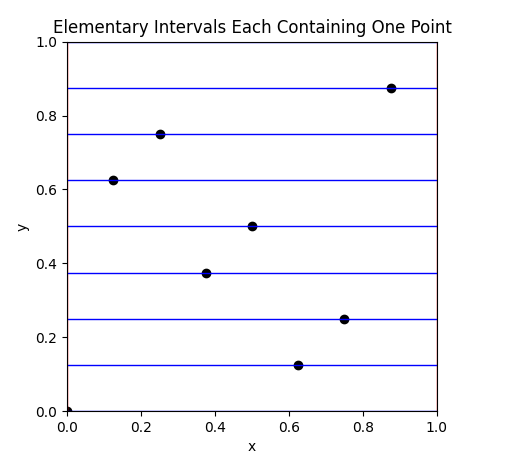
\includegraphics[width=\linewidth]{image.png}
\caption{$(d_1,d_2)=(0,3)$}
\label{first combination}
\end{subfigure}
\hfill
\begin{subfigure}{0.45\textwidth}
\centering
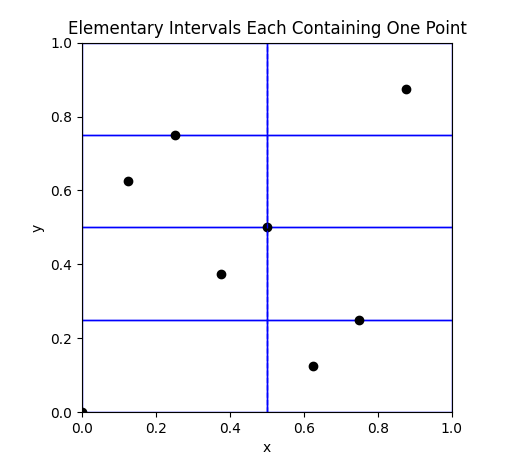
\includegraphics[width=\linewidth]{nets.png}
\caption{$(d_1,d_2)=(1,2)$}
\label{second combination}
\end{subfigure}

\vspace{0.5em}

\begin{subfigure}{0.45\textwidth}
\centering
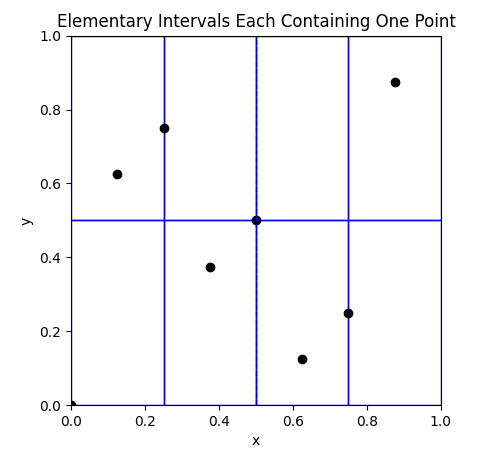
\includegraphics[width=\linewidth]{nets2.png}
\caption{$(d_1,d_2)=(2,1)$}
\label{third combination}
\end{subfigure}
\hfill
\begin{subfigure}{0.45\textwidth}
\centering
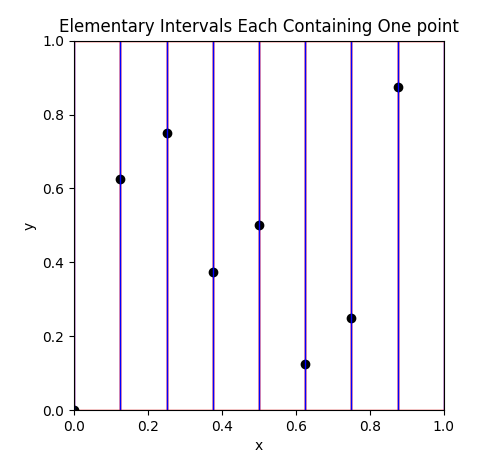
\includegraphics[width=\linewidth]{nets3.png}
\caption{$(d_1,d_2)=(3,0)$}
\label{Fourth combination}
\end{subfigure}
\caption{Elementary Intervals for Different Combinations of \((d_1,d_2)\)}
\end{figure}
\begin{appendixlemma}
  \label{interval of sobol points 1}
Let $\mathcal{P}$ be a $(t,\ell,s)$-net of Sobol Sequences consisting of the points \(x_0,x_1,\ldots,x_{2^{\ell}-1}\), then \(\forall\; x_i\in\mathcal{P} \) such that \(i\neq0,\; x_i\in\Big[\frac{1}{N},1-\frac{1}{N}\Big]\) where \(N=2^{\ell} \)  
\end{appendixlemma}

\begin{proof}
Let  $x_{n}$ be a point in the sequence.From the algorithm presented in this appendix, we write $n$ in its binary representation. Since the largest value of \(n\) is \(2^{\ell}-1\), we need \(\ell\) bits to represent \(n\) in binary thus \(n=n_0+2n_1+\cdot\cdot\cdot 2^{\ell-1}n_{\ell-1}\) then we have \begin{equation}
    x_{n}=n_0v_{1}\oplus n_1v_{2}\oplus\cdot\cdot\cdot\oplus n_{\ell-1}v_{\ell}
\end{equation} so we need the first $\ell$ direction numbers, but \(v_{\ell}=\frac{m_{\ell}}{2^{\ell}}\). From the construction of the algorithm, we know that \(m_{\ell}<2^{\ell}\) thus, we need \(\ell\) bits to represent $m$ in binary hence \(m_{\ell}=m_{0}m_{1}\cdot\cdot\cdot m_{\ell-1}\) then the binary representation of $v_{\ell}$ is that of $m_{\ell}$ after shifting the digits of $m$ $\ell$ times to the right of the binary point hence \(v_{\ell}=0.m_{0}m_{1}\cdot\cdot\cdot m_{\ell-1,i}\)
then \begin{equation}
    x_{n}=n_0v_{1}\oplus n_1v_{2}\oplus\cdot\cdot\cdot\oplus n_{\ell-1}v_{\ell}.
\end{equation}Since all the terms that we are xoring can be represented using $\ell$ bits so $x_{n}$ will have $\ell$ bits in its binary representation so the largest value that $x_{n}$ will have is \begin{equation}
x_{n}=0.11\cdot\cdot\cdot111=\sum_{i=1}^{\ell} \frac{1}{2^i}=\frac{1}{2}\left(\frac{1-(\frac{1}{2})^{\ell}}{1-\frac{1}{2}}\right)=1-\frac{1}{2^{\ell}}=1-\frac{1}{N}
\end{equation}
and the smallest value that $x_{n}$ will have is \begin{equation}
x_{n}=0.0\cdot\cdot\cdot1=\frac{1}{2^{\ell}}=\frac{1}{N}
\end{equation}
note that $x_{n}=0$ cannot result from the xoring operations because all the direction vectors are different. Then $x_{n}\in[\frac{1}{N},1-\frac{1}{N}]\;\forall \;n=1,\ldots,N$ 
\end{proof}

\section{Owen Scrambling and Shifting}

\label{app: Owen Scrambling}
We have motivated the need for the randomization of the Sobol' Sequences throughout this paper, and how Owen Scrambling can lead to a high probability of not getting the problematic 0 point. In this part of the appendix, we present the Owen Scrambling algorithm, we give an example to illustrate the scrambling procedure, and we prove theorem \ref{th:pzero}.
\begin{definition}
 A permutation of the set $\{0,1\}$ is a bijection \(
     \pi : \{0,1\} \longrightarrow \{0,1\}
\).
\end{definition}
 \noindent We are interested in the set $\{0,1\}$ because in Owen scrambling, we will permute the digits of the binary representation of each component of our vector. Since Sobol sequences are in base 2, we are only interested in permutations of $\{0,1\}$. In this case there are only two possible permutations. Let $\Xi$ denote the set of all possible permutations . Then \(\Xi=\{\textit{swap},\mathcal{I}_d\}\) 
where \begin{align*}
\textit{swap} : \{0,1\} &\longrightarrow \{0,1\},
& \textit{swap}(0) &= 1,\quad \text{and}\quad \textit{swap}(1)=0, \\
\mathcal{I}_d : \{0,1\} &\longrightarrow \{0,1\},
& \mathcal{I}_d(0) &= 0,\quad \text{and}\quad \mathcal{I}_d(1)=1.
\end{align*}
In the following we present the Owen Scrambling Algorithm given in \cite{OwenArtB.1995RP(m}.\\
\noindent\textbf{Owen Scrambling Algorithm :} 
Let $(A_i)$ be a $(t,m,s)$-net or a $(t,s)$-sequence in base $b$. The $i$'th term in the sequence is denoted $A_i=(A_i^1,A_i^2,\cdot\cdot\cdot,A_i^s)$. We can write the components of $A_i$ in their base $b$ expansion \begin{equation}
    A_i^j=\sum_{k=1}^{\infty}a_{ijk}b^{-k}
\end{equation} where $0\leq a_{ijk}<b$ for all $i,j,k$. A randomized version of $(A_i)$ is a sequence $(X_i)$ with elements $X_i=(X_i^1,X_i^2,\cdot\cdot\cdot,X_i^s)$ written as \begin{equation}
    X_i^j=\sum_{k=1}^{\infty}x_{ijk}b^{-k}
\end{equation} with $x_{ijk}$ defined in terms of random permutations of $a_{ijk}$
\begin{align*}
x_{ij1}&=\pi_j(a_{ij1})\\
x_{ij2}&=\pi_{ja_{ij1}}(a_{ij2})\\
x_{ij3}&=\pi_{ja_{ij1}a_{ij2}}(a_{ij3})\\
\vdots\\
x_{ijk}&=\pi_{ja_{ij1}a_{ij2}\cdots a_{ijk-1}}(a_{ijk})\\
\vdots
\end{align*}
\noindent each of these permutations is distributed uniformly over the set of all possible permutations. The same set of permutations permutes the same digits of the same component of every vector.In theory, we should keep on scrambling all the digits infinitely, but in practice this is not possible so we choose a specific amount of extra bits that we want to scramble. The more bits we choose, the better.In he following, we discuss the maximum number of bits such that no error comes from approximating the number when it is represented in IEEE-754 double precision format.In IEEE-754 double precision format, we represent a number $p$ as \(p=s_0e_0e_1\cdot\cdot\cdot e_7m_0\cdot\cdot\cdot m_{51}\) where $s_0$ is the sign bit, $e_0e_1\cdot\cdot\cdot e_7$ are the exponent and $m_0\cdot\cdot\cdot m_{51}$ represent the mantissa,
and there is an implied one so that we get \begin{equation}
    p=\pm 1.M\times 2^{ E-1023}
\end{equation}
the exponent is represented in excess 1023.Since all the numbers that we are generating are in $ [0,1)$, there is no integer part. This means that with the implied one, we can have a maximum of 53 digits after the binary point in fixed point representation. In a $(t,m,s)$ net we have $m$ digits after the binary point, so we can scramble $s=53-m$ additional bits without round off errors in the floating point representation.If we want to shift our points , we need to add $\frac{1}{2^{s+m}}$ to our number so to avoid overflow, we can scramble at most $s=52-m$.However, our numerical computations show that much less bits are needed for this scrambling procedure to get accurate results.\\
\noindent\textbf{Example B.1 }Lets scramble the first four points of the Sobol sequence in $\mathbb{R}^2$ which are\begin{equation}
    \mathcal{P}=\{(0,0),(0.5,0.5),(0.75,0.25),(0.25,0.75)
\end{equation} with one extra bit .\\
First, we permute the first component of each vector.We have to randomly choose the required permutations for each component of our vectors. We randmoly choose the following \begin{table}[H]
\centering
\begin{tabular}{ccccccc}
\hline
$\pi_{1}$ & $\pi_{10}$ & $\pi_{11}$ & $\pi_{100}$ & $\pi_{101}$ & $\pi_{110}$ & $\pi_{111}$ \\
\hline
$\textit{swap}$ 
& $\textit{swap}$ 
& $\mathcal{I}_d$ 
& $\mathcal{I}_d$ 
& $\mathcal{I}_d$ 
& $\textit{swap}$ 
& $\mathcal{I}_d$ \\
\hline
\end{tabular}
\caption{permutations associated with binary prefixes for the first component of each vector}
\end{table}
\noindent The following tables show the permutations that are happening; we have underlined the digit that we are permuting.
\begin{table}[H]       % Optional: for floating table with positioning
  \centering            % Center the table
  \caption{Permuting The First Digit in the First Component of Each Vector}
  \label{tab:1}
  \begin{tabular}{|c|c|c|c|c|}  % 5 centered columns with vertical lines
    \hline
    n & Sobol Point & Prefix & required permutation & result \\ \hline
    0 & 0.\underline{0}00 & no prefix & $\pi_1$ & $\pi_1(0)=1$ \\ \hline
    1 & 0.\underline{1}00 & no prefix & $\pi_1$ & $\pi_1(1)=0$ \\ \hline
    2 & 0.\underline{1}10 & no prefix & $\pi_1$ & $\pi_1(1)=0$ \\ \hline
    3 & 0.\underline{0}10 & no prefix & $\pi_1$ & $\pi_1(0)=1$ \\ \hline
  \end{tabular}
\end{table}
\begin{table}[H]       % Optional: for floating table with positioning
  \centering            % Center the table
  \caption{Permuting The Second Digit in the First Component of Each Vector}
  \label{tab:2}
  \begin{tabular}{|c|c|c|c|c|}  % 5 centered columns with vertical lines
    \hline
    n & Sobol Point & Prefix & required permutation & result \\ \hline
    0 & 0.0\underline{0}0 & 0 & $\pi_{10}$ & $\pi_{10}(0)=1$ \\ \hline
    1 & 0.1\underline{0}0 & 1 & $\pi_{11}$ & $\pi_{11}(0)=0$ \\ \hline
    2 & 0.1\underline{1}0 & 1 & $\pi_{11}$ & $\pi_{11}(1)=1$ \\ \hline
    3 & 0.0\underline{1}0 & 0 & $\pi_{10}$ & $\pi_{10}(1)=0$ \\ \hline
  \end{tabular}
\end{table}
\begin{table}[H]       % Optional: for floating table with positioning
  \centering            % Center the table
  \caption{Permuting The Third Digit in the First Component of Each Vector}
  \label{tab:3}
  \begin{tabular}{|c|c|c|c|c|}  % 5 centered columns with vertical lines
    \hline
    n & Sobol Point & Prefix & required permutation & result \\ \hline
    0 & 0.00\underline{0} & 00 & $\pi_{100}$ & $\pi_{100}(0)=0$ \\ \hline
    1 & 0.10\underline{0} & 10 & $\pi_{110}$ & $\pi_{110}(0)=1$ \\ \hline
    2 & 0.11\underline{0} & 11 & $\pi_{111}$ & $\pi_{111}(0)=0$ \\ \hline
    3 & 0.01\underline{0} & 01 & $\pi_{101}$ & $\pi_{101}(0)=0$ \\ \hline
  \end{tabular}
\end{table}
\noindent The resulting first components of each vector are \begin{equation}
    (0.110)_2=0.75\;\;\;(0.001)_2=0.125\;\;\;(0.010)_2=0.25\;\;\;(0.100)_2=0.5
\end{equation}
For the second component, we randomly choose the following permutations.
\begin{table}[H]
\centering
\begin{tabular}{ccccccc}
\hline
$\pi_{2}$ & $\pi_{20}$ & $\pi_{21}$ & $\pi_{200}$ & $\pi_{201}$ & $\pi_{210}$ & $\pi_{211}$ \\
\hline
$\mathcal{I}_d$ 
& $\textit{swap}$ 
& $\textit{swap}$ 
& $\mathcal{I}_d$ 
& $\textit{swap}$ 
& $\mathcal{I}_d$ 
& $\mathcal{I}_d$ \\
\hline
\end{tabular}
\caption{permutations associated with binary prefixes for the second component of each vector}
\end{table}
\noindent Similar to permuting the first component, we underline the digit that we are permuting.
\begin{table}[H]       % Optional: for floating table with positioning
  \centering            % Center the table
  \caption{Permuting The First Digit in the Second Component of Each Vector}
  \label{tab:4}
  \begin{tabular}{|c|c|c|c|c|}  % 5 centered columns with vertical lines
    \hline
    n & Sobol Point & Prefix & required permutation & result \\ \hline
    0 & 0.\underline{0}00 & no prefix & $\pi_2$ & $\pi_2(0)=0$ \\ \hline
    1 & 0.\underline{1}00 & no prefix & $\pi_2$ & $\pi_2(1)=1$ \\ \hline
    2 & 0.\underline{0}10 & no prefix & $\pi_2$ & $\pi_2(0)=0$ \\ \hline
    3 & 0.\underline{1}10 & no prefix & $\pi_2$ & $\pi_2(1)=1$ \\ \hline
  \end{tabular}
\end{table}
\begin{table}[H]       % Optional: for floating table with positioning
  \centering            % Center the table
  \caption{Permuting The Second Digit of the Second Component of Each Vector}
  \label{tab:5}
  \begin{tabular}{|c|c|c|c|c|}  % 5 centered columns with vertical lines
    \hline
    n & Sobol Point & Prefix & required permutation & result \\ \hline
    0 & 0.0\underline{0}0 & 0 & $\pi_{20}$ & $\pi_{20}(0)=1$ \\ \hline
    1 & 0.1\underline{0}0 & 1 & $\pi_{21}$ & $\pi_{21}(0)=1$ \\ \hline
    2 & 0.0\underline{1}0 & 0 & $\pi_{20}$ & $\pi_{20}(1)=0$ \\ \hline
    3 & 0.1\underline{1}0 & 1 & $\pi_{21}$ & $\pi_{21}(1)=0$ \\ \hline
  \end{tabular}
  
\end{table}
\begin{table}[H]       % Optional: for floating table with positioning
  \centering            % Center the table
  \caption{Permuting The Third  Digit of the Second Component of Each Vector}
  \label{tab:6}
  \begin{tabular}{|c|c|c|c|c|}  % 5 centered columns with vertical lines
    \hline
    n & Sobol Point & Prefix & required permutation & result \\ \hline
    0 & 0.00\underline{0} & 00 & $\pi_{200}$ & $\pi_{200}(0)=0$ \\ \hline
    1 & 0.10\underline{0} & 10 & $\pi_{210}$ & $\pi_{210}(0)=0$ \\ \hline
    2 & 0.01\underline{0} & 01 & $\pi_{201}$ & $\pi_{201}(0)=1$ \\ \hline
    3 & 0.11\underline{0} & 11 & $\pi_{211}$ & $\pi_{211}(0)=0$ \\ \hline
  \end{tabular}
  
\end{table}
The resulting second components of each vector are \begin{equation}
    (0.010)_2=0.25\;\;\;(0.110)_2=0.75\;\;\;(0.001)_2=0.125\;\;\;(0.100)_2=0.5
\end{equation}
The resulting points after scrambling are \begin{equation}
    \mathcal{P}_{\text{s}}=\{(0.75,0.25),(0.125,0.75),(0.25,0.125),(0.5,0.5)\}
\end{equation}
As we can see, the point $(0,0)$ has been eliminated.\\
\textit{Proof of Theorem} \ref{th:pzero}
\begin{proof}
Consider the following event \(A_i \text{ : } \text{"}x_i \text{ will become 0 after we permute its digits "}\).
We will show that \begin{equation}
    \mathbb{P}(A_i \cap A_j)=0 \qquad i\neq j.
\end{equation}
Lets find the probability that $x_i$ will go to 0. Writing $x_i$ in its binary representation with the extra bits we get \begin{equation}
    x_i=\sum_{\ell=1}^{k+m}a_{i\ell}2^{-\ell}
\end{equation}
for $x_i$ to become zero we need $\pi_1(a_{i1})=0$ . If $a_{i1}=1$ we need $\pi_1=\textit{swap}$, and if $a_{i1}=0$ we need $\pi_1=\mathcal{I}_d$. In both cases, we need $\pi_1$ to be a specific permutation which has probability half. Similarly for all $a_{i\ell}\;, 1\leq \ell\leq m+k$ so \begin{equation}
    \mathbb{P}(A_i)=\frac{1}{2}\times \frac{1}{2}\cdot\cdot\cdot\times\frac{1}{2}=\frac{1}{2^{m+k}}=\frac{1}{2^{k}N}
\end{equation} 
For $x_j$ to become zero, we write down the binary representation of $x_j$ \begin{equation}
    x_j=\sum_{\ell=1}^{m+k}a_{j\ell}2^{-\ell}
\end{equation}
since $x_i \neq x_j, \; \exists\; \tau $ such that $a_{i\tau}\neq a_{j\tau} $.Let $\tau$ be the first digit where $x_i$ and $x_j$ differ, so by the construction of the Owen Scrambling algorithm $a_{it}=a_{jt}\; \forall\;  0\leq t< \tau $
then we have \begin{align*}
\pi_1&=\pi_1\\
\pi_{1a_{i1}}&=\pi_{1a_{j1}}\\
\pi_{1a_{i1}a_{i2}}&=\pi_{1a_{j1}a_{j2}}\\
&\vdots\\
\pi_{1a_{i1}a_{i2}\cdot\cdot\cdot a_{i\tau-1}} &=\pi_{1a_{j1}a_{j2}\cdot\cdot\cdot a_{j\tau-1}} \\
\end{align*}
assume WLOG that $a_{i\tau}=0$ then $a_{j\tau}=1$, for $x_i$ to go to 0 we need $\pi_{1a_{i1}a_{i2}\cdot\cdot\cdot a_{i\tau-1}}=\mathcal{I}_d$ , and for $x_j$ to go to 0, we need $\pi_{1a_{j1}a_{j2}\cdot\cdot\cdot a_{j\tau-1}}=\textit{swap}$ but this cannot happen because $\pi_{1a_{i1}a_{i2}\cdot\cdot\cdot a_{i\tau-1}} =\pi_{1a_{j1}a_{j2}\cdot\cdot\cdot a_{j\tau-1}}$ thus \(\mathbb{P}(A_j|A_i)=0\) then\begin{equation}
    \mathbb{P}(A_i \cap A_j)=\mathbb{P}(A_i)\mathbb{P}(A_j|A_i)=\frac{1}{2^{k}N} \times 0=0
\end{equation}
This shows that at most one point can map to 0.
Since we have $N$ points, the probability that a point will become zero is $\frac{1}{2^{k}N} \times N=\frac{1}{2^{k}}$.
Now consider the following events E : "no point maps to zero after scrambling ", F:"at least one points maps to zero after scrambling", and W :"one point maps to zero after scrambling". Since at most one point can map to zero we have $\mathbb{P}(\text{F})=\mathbb{P}(\text{W})$ and $\mathbb{P}(\text{W})=\frac{1}{2^{k}}$ therefore  \begin{equation}
\mathbb{P}(\text{E})=1-\mathbb{P}(\text{F})
=1-\mathbb{P}(\text{W}) 
=1-\frac{1}{2^{k}}
\end{equation}
\end{proof}
\begin{appendixtheorem}
  \label{th:shift}
Let $\mathcal{P}=\{\mathbf{x}_0,\cdot\cdot\cdot,\mathbf{x}_{N-1}\}$ be a point set in $[0,1)^s$ with star discrepancy $D_N^{\ast}(\mathcal{P})$. Let $\mathbf{x}_n=(x_{n,1},x_{n,2},\cdot\cdot\cdot x_{n,s})$ for $0\leq n\leq N-1$ and let $\delta_{n,i}, 0\leq n\leq N-1$ $1\leq i\leq s$ be non-negative reals with $\delta_{n,i}<\epsilon$ such that $x_{n,i} + \delta_{n,i}<1$ for all $0\leq n\leq N-1$ and  $1\leq i\leq s$. Then for the star discrepancy $D_N^{\ast}(\mathcal{P}^{\text{s}})$ of the shifted point set $\mathcal{P}^{\text{s}}=\{\mathbf{x}^{\text{s}}_0,\mathbf{x}^{\text{s}}_1,\cdot\cdot\cdot, \mathbf{x}^{\text{s}}_n\}$ with ${x}^{\text{s}}_{n,i}=x_{n,i}+\delta_{n,i}$ for all $0\leq n\leq N-1$ and  $1\leq i\leq s$, we have \begin{equation}
\lvert D_N^{\ast}(\mathcal{P}) - D_N^{\ast}(\widetilde{\mathcal{P}})\rvert \leq \epsilon s
\end{equation}
\end{appendixtheorem}
\noindent The proof can be found in \cite{DickJosef2010D}.
\begin{appendixlemma}
\label{lem:r1}
Let $\mathcal{P}_{\text{scrambled}}$ be the same as in Theorem \ref{thm: approximate scrambling} then 
\(\forall \;x_i\in\mathcal{P}_{\text{scrambled}}\;, i\neq 0 \;,\; x_{i}\in\left[\frac{1}{2^{k}n},1-\frac{1}{2^{k}n}\right]
\)
\end{appendixlemma}
\begin{proof}
From Lemma \ref{interval of sobol points 1}, we know that before scrambling, the components of each vector have $m$ bits in their binary represenation. With $k$ extra bits, we have $m+k$ bits in the binary represenation of each point; the proof follows in the same way as in Lemma \ref{interval of sobol points 1} and using the fact that $2^{m+k}=2^{k}n$
\end{proof}


\section{Asymptotic Expansion}
For asymptotic expansion, we rely on definition present in Copson (1965) \cite{Copson_1965} which is the refinement of Poincare definition.
\begin{appendixdefinition}[Asymptotic Scale]\label{def:asymptotic-scale}
Let \( \varphi_n(x) \) be a sequence of continuous functions on a domain \(D \) and \( a \) a limit point of \( D \). Then the sequence is said to be an asymptotic scale if \( \forall n \in \mathbb{N} \),
\[
\varphi_{n+1}(x) = o(\varphi_n(x)) \qquad \text{ as }  x \to a.
\]
\end{appendixdefinition}

\begin{appendixdefinition}[Poincare Definition of Asymptotic Expansion]\label{def:asymptotic-expansion}
Let \( f \) a continuous function on the domain of a fixed asymptotic scale \( \{ \varphi_n(x)\} \).
Then \( f \) has an asymptotic expansion of order \(N\in\mathbb{N}\) with respect to the asymptotic scale as a formal series as \(x \to a \),
\[
f(x)-\sum_{n=0}^{N-1} a_n\varphi_n(x) = o( \varphi_{N-1}(x)) \quad \text{as } x \to a.
\]

A slightly stronger version (for that specific \(N\in\mathbb{N}\)) is:
\[
f(x)-\sum_{n=0}^{N-1}a_n\varphi_n(x)=O(\varphi_{N}(x)) \quad\text{as }x\to a.
\]
However, if one of the above holds \(\forall N\in\mathbb{N}\), then the above definitions become equivalent, and we write
\[ 
f(x) \sim \sum_{n=0}^\infty a_n \varphi_n(x).
\]
If such an asymptotic expansion exists for a fixed asymptotic scale, then it is \emph{unique} and its coefficients are recursively given by:
\[
a_{N} = \lim_{x \to a} \frac{f(x)- \sum_{n=1}^{N-1} a_n \varphi_n(x) }{\varphi_{N}(x)} \quad \text{for }N\ge1.
\]
Its partial sum
\[
\sum_{n=0}^{N-1} a_n \varphi_n(x)
\]
is an approximation to \( f(x) \) with error \( O(\varphi_N)\) as \( x \to a\).\\
\textit{Note:} The definition is \(0\)-indexed; however, \(1\)-indexed notation will be used when convenient.
\end{appendixdefinition}

\begin{proof}We only prove the equivalence of the remainder conditions when the expansion holds to all orders. For simplicity, assume that asymptotic scale \{\(\varphi_n(x)\)\} eventually nonzero as \(x\to a\) \(\forall n\in\mathbb{N}\).\\
(\(\Rightarrow\)) Assume that, for each \(N \in \mathbb{N}\),
\[
f(x)-\sum_{n=0}^{N-1} a_n\varphi_n(x) = o( \varphi_{N-1}(x)) \quad \text{as } x \to a,
\]
\[
f(x)-\sum_{n=0}^{N-1} a_n\varphi_n(x)-a_{N}\varphi_{N}(x)= o( \varphi_{N}(x)) \quad \text{as } x \to a,
\]
\[
\implies\lim_{x\to a}{\frac{f(x)-\sum_{n=0}^{N-1} a_n\varphi_n(x)-a_{N}\varphi_{N}(x)}{\varphi_{N}(x)}}=0
\]
\[
\implies \lim_{x\to a}\frac{f(x)-\sum_{n=0}^{N-1} a_n\varphi_n(x)}{\varphi_{N}(x)}=a_{N}<\infty.
\]
\[
\implies f(x)-\sum_{n=0}^{N-1}a_n\varphi_n(x)= O(\varphi_{N}(x)) \quad\text{as }x\to a.
\]

(\(\Leftarrow\)) Conversely, since \(\varphi_N(x)=o(\varphi_{N-1}(x))\), the bound
\(O(\varphi_N(x))\) immediately implies \(o(\varphi_{N-1}(x))\).
Thus, when the expansion holds for all $N$, the two formulations of the
remainder are equivalent.%
\end{proof}
\textit{Note:} Two distinct functions may yield identical asymptotic expansions, i.e. the they share the same coefficients for some fixed asymptotic scale.
\begin{appendixexample}\label{ex:Cauchy-asymp-exp}
    The coefficients of  asymptotic expansion of Cauchy distribution \(f(x)=f(x\,|\,1,0;0)\) as \(x\to\infty\) for the fixed asymptotic scale \(\{x^{-(1+n)}\}\) may be readily obtained since we know that:
\begin{equation*}
f(x\,|\,1,0;0)=\frac{1}{\pi}\frac{1}{1+x^2}=\frac{1}{\pi}\sum_{n=1}^\infty\frac{(-1)^{n+1}}{x^{2n}} \text{ for }x>1.
\end{equation*}
It can be easily verified that the above series expansion satisfy the definition for the asymptotic expansion as \(x\to\infty\) with asymptotic scale \(\{x^{-2n}\}\):
\begin{equation}
   f(x\,|\,1,0;0)\sim\frac{1}{\pi}\sum_{n=1}^\infty(-1)^{n+1}x^{-2n} \text{ as }x\to\infty. 
\end{equation}
It may also be rewritten w.r.t. asymptotic scale \(\{x^{-(1+n)}\}\) as:
\begin{equation*}
    f(x\,|\,1,0;0)=\frac{1}{\pi}\frac{1}{1+x^2}\sim\frac{1}{\pi}\sum_{n=1}^\infty{a_n}x^{-(1+n)} \quad \text{as }x\to\infty
\end{equation*}
where \(a_n=\sin{\!\left(\!\frac{\pi n}{2}\!\right)}\) (the even coefficients are 0).\\
The asymptotic expansion of L\'evy distribution \(f(x)=f(x\,|\,0.5,1;0)\) as \(x\to\infty\) is also available.\
\end{appendixexample}

\begin{appendixtheorem}[Zolotarev, Equation (2.4.8)]\label{th:series_expansion_1}
If \(\alpha<1\), for any admissable \(\beta\) and any \(x>0\),
\begin{equation}
    g(x,\alpha,\beta)=\frac{1}{\pi}\sum_{n=1}^\infty
    (-1)^{n-1}\frac{\Gamma(n\alpha+1)}{n!}
    \sin(\pi n\rho \alpha)x^{-(1+n\alpha)}
\end{equation}
where \(\rho=\frac{1+\theta}{2}\) and \(\)
\end{appendixtheorem}

\begin{appendixtheorem}[Zolotarev, Theorem 2.5.1, Corollary~2]\label{th:series_expansion_2}
Let \(\alpha>1\) and \(\beta\neq-1\). Then, as \(x\to\infty\), the stable PDF admits the asymptotic expansion
\begin{equation}
g(x;\alpha,\beta)
\sim
\frac{\alpha}{\pi}
\sum_{n=1}^{\infty}
\frac{\Gamma(\alpha n)}{\Gamma(n)}
\sin\!\left(\frac{\pi n}{2}(2-\alpha)(1+\beta)\right)
x^{-1-n\alpha}.
\label{eq:zolo_alpha_gt_1_asymptotic}
\end{equation}
\end{appendixtheorem}


\begin{appendixtheorem}[Zolotarev, Theorem~2.5.4]\label{th:series_expansion_3}
Let \(\alpha=1\) and \(\beta\neq-1\). Then, as \(x\to\infty\), the stable
PDF admits the asymptotic expansion
\begin{equation}
g(x;1,\beta)
\sim
\frac{1}{\pi}
\sum_{n=1}^{\infty}
\frac{1}{n!}\,P_n(\log x)\,x^{-n-1},
\label{eq:zolo_alpha1_asymptotic}
\end{equation}
where $P_n$ is a polynomial of degree $n$ given by
\begin{equation}
P_n(y)=\sum_{l=0}^{n} r_{l n}\, y^{l},
\end{equation}
and the coefficients $r_{l n}$ are defined by
\begin{equation}
r_{l n}
=
\sum_{m=l}^{n}
\binom{n}{m}\binom{m}{l}
(-1)^{m-l}
\Gamma(m-l)\Gamma(1+n)\,
\beta^{m}
\left(\frac{\pi}{2}(1+\beta)\right)^{n-m}
\sin\!\left(\frac{\pi}{2}(n-m)\right).
\end{equation}
\end{appendixtheorem}



\iffalse
\begin{appendixtheorem}[Composition at singular limit points]
Let $f(x)\to L$ as $x\to a$, where $L\in\{0,+\infty,-\infty\}$, and suppose that
$f$ admits an asymptotic expansion of infinite order
\[
f(x)\sim \sum_{n=1}^\infty a_n \varphi_n(x),
\qquad x\to a,
\]
with respect to an asymptotic scale $\{\varphi_n\}$ satisfying
\[
\varphi_{n+1}(x)=o(\varphi_n(x)).
\]

Let $g\in C^\infty$ on a punctured neighborhood of $L$ and assume that $L$ is a
singular point of $g$. Suppose further that for all $k\ge0$,
\[
g^{(k)}(y)
=
O\!\left(\frac{g(y)}{|y|^k}\right),
\qquad y\to L.
\]

Then $g(f(x))$ admits an asymptotic expansion of infinite order as $x\to a$,
whose asymptotic scale is induced by the leading term of the expansion of $f$.
\end{appendixtheorem}

\begin{appendixtheorem}[Asymptotic expansion of $g(f(x))$ at a singular point]
Let $f(x)\to0^+$ as $x\to a$ and suppose that $f$ admits an asymptotic expansion
of infinite order
\[
f(x)\sim \sum_{n=1}^\infty a_n \varphi_n(x)
\qquad \text{as } x\to a,
\]
with respect to an asymptotic scale $\{\varphi_n\}$ satisfying
\[
\varphi_{n+1}(x)=o(\varphi_n(x)),
\qquad \varphi_1(x)\to0^+,
\qquad a_1\neq0.
\]

Assume that $g$ is singular at $0$ and regularly varying at $0$, i.e.
\[
g(y)=y^{\gamma}L(y), \qquad y\to0^+,
\]
for some $\gamma\in\mathbb{R}$ and some slowly varying function $L$.

Then, writing
\[
f(x)
=
a_1\varphi_1(x)\bigl(1+\varepsilon(x)\bigr),
\qquad
\varepsilon(x)
\sim
\sum_{n\ge2}\frac{a_n}{a_1}\frac{\varphi_n(x)}{\varphi_1(x)},
\]
the composition $g(f(x))$ admits the asymptotic expansion
\[
g(f(x))
\sim
g\bigl(a_1\varphi_1(x)\bigr)
\sum_{k=0}^\infty
\binom{\gamma}{k}\,\varepsilon(x)^k,
\qquad \text{as }x\to a.
\]

Equivalently,
\[
g(f(x))
\sim
g\bigl(a_1\varphi_1(x)\bigr)
\left[
1
+
\gamma\sum_{n\ge2}\frac{a_n}{a_1}\frac{\varphi_n(x)}{\varphi_1(x)}
+
\frac{\gamma(\gamma-1)}{2}
\left(\sum_{n\ge2}\frac{a_n}{a_1}\frac{\varphi_n(x)}{\varphi_1(x)}\right)^2
+\cdots
\right].
\]
\end{appendixtheorem}

\begin{appendixcorollary}[Entropy kernel (Copson form)]
Let $\{\varphi_n\}_{n\ge1}$ be an asymptotic scale as $x\to a$, i.e.
\[
\varphi_{n+1}(x)=o(\varphi_n(x)),
\qquad x\to a,
\]
with $\varphi_1(x)\to0^+$.
Assume that
\[
f(x)\sim \sum_{n=1}^\infty a_n \varphi_n(x),
\qquad x\to a,
\]
in the sense of Copson, meaning that for each $N\ge1$,
\[
f(x)-\sum_{n=1}^N a_n\varphi_n(x)=O\!\left(\varphi_{N+1}(x)\right).
\]

Then the entropy kernel $g(y)=y\log y$ satisfies
\[
\begin{aligned}
f(x)\log f(x)
={}&
a_1\varphi_1(x)\log\varphi_1(x)
+
a_2\varphi_2(x)\log\varphi_1(x)
\\
&+
a_1\varphi_1(x)\log a_1
+
a_2\varphi_2(x)
+
O\!\left(\varphi_3(x)\log\varphi_1(x)\right),
\qquad x\to a.
\end{aligned}
\]

More generally, for each $N\ge1$,
\[
f(x)\log f(x)
-
\sum_{n=1}^N
\left(
a_n\varphi_n(x)\log\varphi_1(x)
+
a_n\varphi_n(x)\mathbf{1}_{\{n=1\}}\log a_1
\right)
=
O\!\left(\varphi_{N+1}(x)\log\varphi_1(x)\right).
\]
\end{appendixcorollary}
\fi

\end{appendices}
\end{document}
